\documentclass[acmsmall,screen,review,anonymous]{acmart}

%\documentclass[sigplan,screen]{acmart}

\usepackage{graphicx}
\usepackage{float}
\usepackage{algorithm}
\usepackage{algpseudocode}
\usepackage{amsmath,amsfonts,mathtools,newtxmath}
\usepackage{balance}
\usepackage{listings}
\usepackage{xcolor}
\usepackage{multirow}
\usepackage{booktabs}
\usepackage{tabularx}
\usepackage{adjustbox}
\usepackage{algorithm2e,subcaption}
\usepackage{enumitem,microtype,pgfplots,pgfplotstable,placeins,tikz}
\usepackage{hyperref}
\usetikzlibrary{shapes,arrows.meta,positioning,shadows,backgrounds,fit,calc,decorations.pathreplacing}
\pgfplotsset{compat=1.18}
\setlist[itemize]{leftmargin=*,itemsep=2pt,topsep=3pt,parsep=0pt}
\setlist[enumerate]{leftmargin=*,itemsep=2pt,topsep=3pt,parsep=0pt}


% Unified ModernPDE / ACM TACO visual palette (use ONLY these):
%   chartBlue / colorLive      RGB 41,128,185
%   chartGreen / colorMostlyLive RGB 39,174,96
%   chartOrange                RGB 243,156,18
%   chartRed / colorDead       RGB 192,57,43
%   chartPurple                RGB 142,68,173
%   chartTeal                  RGB 26,188,156
%   chartDarkBlue              RGB 31,78,121
%   colorMostlyDead            RGB 230,126,34
%   colorPartiallyDead         RGB 241,196,15
%   codeBg                     RGB 248,249,250
% ---- Colors (unified TACO palette) ----
\definecolor{colorDead}{RGB}{192,57,43}
\definecolor{colorMostlyDead}{RGB}{230,126,34}
\definecolor{colorPartiallyDead}{RGB}{241,196,15}
\definecolor{colorMostlyLive}{RGB}{39,174,96}
\definecolor{colorLive}{RGB}{41,128,185}
\definecolor{chartBlue}{RGB}{41,128,185}
\definecolor{chartGreen}{RGB}{39,174,96}
\definecolor{chartOrange}{RGB}{243,156,18}
\definecolor{chartRed}{RGB}{192,57,43}
\definecolor{chartPurple}{RGB}{142,68,173}
\definecolor{chartTeal}{RGB}{26,188,156}
\definecolor{chartDarkBlue}{RGB}{31,78,121}
\definecolor{codeBg}{RGB}{248,249,250}
\definecolor{codeKeyword}{RGB}{142,68,173}
\definecolor{codeType}{RGB}{41,128,185}
\definecolor{codeComment}{RGB}{39,174,96}
\definecolor{codeString}{RGB}{230,126,34}
\definecolor{codeNum}{RGB}{192,57,43}

% ---- Listings (colored code) ----
\lstset{
  basicstyle=\ttfamily\footnotesize,
  backgroundcolor=\color{codeBg},
  keywordstyle=\color{codeKeyword}\bfseries,
  commentstyle=\color{codeComment}\itshape,
  stringstyle=\color{codeString},
  numberstyle=\color{codeNum}\tiny,
  numbers=left, numbersep=6pt,
  frame=single, rulecolor=\color{chartDarkBlue},
  breaklines=true, tabsize=2, showstringspaces=false,
  morekeywords={void,if,else,Metadata,Txn,STANDARD},
  morecomment=[l]{//}
}

% ---- Algorithm2e (publication style) ----
\usepackage{tcolorbox}
\tcbuselibrary{skins,breakable}
\SetAlFnt{\small\ttfamily}
\SetAlCapFnt{\small\bfseries}
\SetAlCapNameFnt{\small\bfseries}
\SetAlgoLined
\SetAlgoCaptionSeparator{.~}
\LinesNumbered
\DontPrintSemicolon
\SetKwComment{Comment}{/*~}{~*/}
\SetKwInOut{Input}{Input}
\SetKwInOut{Output}{Output}
\SetKwFor{ForEach}{for each}{do}{end}
\SetKwFunction{EnumPaths}{EnumerateRelevantPaths}
\SetKwFunction{CompLive}{ComputeLiveness}
\SetKwFunction{ExtractCtx}{ExtractContext}
\SetKwFunction{Equiv}{Equivalent}
\SetKwFunction{AnalyzeFn}{AnalyzeFunction}
\SetKwFunction{ResolveCtx}{ResolveContext}
\SetKwFunction{CreateObj}{CreateSymbolicObject}
\SetKwFunction{ResolveObj}{ResolveObject}
\SetKwFunction{GetField}{GetField}
\SetKwFunction{GetVal}{GetValue}
\SetKwFunction{Update}{Update}
\SetKwFunction{Propagate}{Propagate}
\newtcolorbox{algobox}{
  colback=codeBg, colframe=chartDarkBlue,
  boxrule=0.9pt, arc=2pt, boxsep=2pt,
  left=5pt, right=5pt, top=2pt, bottom=2pt,
  enhanced, breakable
}

%%
%% \BibTeX command to typeset BibTeX logo in the docs
\AtBeginDocument{%
  \providecommand\BibTeX{{%
    Bib\TeX}}}
\setcopyright{none}
\copyrightyear{2026}
\acmYear{2026}
\acmDOI{Y}
%% These commands are for a PROCEEDINGS abstract or paper.
\acmJournal{TACO}
\acmVolume{x}
\acmNumber{y}
\acmArticle{z}
\acmMonth{12}
\received{2026-x-x}
\received[accepted]{2026-x-x}
  
%%
%%  Uncomment \acmBooktitle if the title of the proceedings is different
%%  from ``Proceedings of ...''!
%%
%%\acmBooktitle{Woodstock '18: ACM Symposium on Neural Gaze Detection,
%%  June 03--05, 2018, Woodstock, NY}
\acmISBN{979-8-4007-1921-9/25/06}
% ---- Float / caption polish (ACM TACO) ----
\setlength{\abovecaptionskip}{4pt}
\setlength{\belowcaptionskip}{2pt}
\setlength{\textfloatsep}{10pt plus 2pt minus 2pt}
\setlength{\floatsep}{8pt plus 2pt minus 2pt}
\setlength{\intextsep}{8pt plus 2pt minus 2pt}
\captionsetup{
  font=small,
  labelfont=bf,
  labelsep=period,
  justification=justified,
  singlelinecheck=false,
  skip=4pt
}
\captionsetup[subfigure]{font=scriptsize,labelfont=bf,justification=centering}
\captionsetup[table]{position=top,skip=3pt}
\captionsetup[figure]{position=bottom,skip=4pt}

% ---- Autoref names (ACM TACO style) ----
\providecommand{\figureautorefname}{Figure}
\providecommand{\tableautorefname}{Table}
\providecommand{\algorithmautorefname}{Algorithm}
\providecommand{\sectionautorefname}{Section}
\providecommand{\subsectionautorefname}{Section}
\providecommand{\equationautorefname}{Equation}




\begin{document}
\title{ModernPDE: A Scalable Framework for Interprocedural Path-Aware Partial Dead Code Elimination}

\author{Mehran Alidoost Nia}
\orcid{0000-0002-7274-9569}
\affiliation{%
  \institution{Faculty of Computer Science and Engineering, \\Shahid Beheshti University}
  \city{Tehran}
  \country{Iran}
}
\email{alidoostnia@sbu.ac.ir}





\renewcommand{\shortauthors}{}

%%
%% The abstract is a short summary of the work to be presented in the
%% article.
\begin{abstract}
Partial dead code elimination (PDE) removes computations that are live on some execution paths and dead on others. Scaling PDE to large interprocedural programs remains difficult because of path explosion, calling-context growth, and imprecise heap modeling. This paper presents \textsc{ModernPDE}, a modular static-analysis framework that combines field-sensitive dataflow analysis, context-sensitive call-graph construction, and path-aware classification. Scalability is obtained through result caching, lazy path enumeration, incremental updates, sparse propagation, and priority-based worklist scheduling. We evaluate the framework on 19 programs ranging from 200 to 50\,000 lines of code. \textsc{ModernPDE} attains 96.2\,\% precision and 91.4\,\% recall, outperforming intraprocedural PDE (72.3\,\%\,/\,61.7\,\%) and summary-based PDE (85.1\,\%\,/\,74.6\,\%). Relative to an exhaustive path baseline, analysis time decreases by 78\,\%, and scalability tests exhibit near-linear growth up to 100\,000 lines (extrapolated). Across the studied programs, 42.1\,\% of variables are partially dead, underscoring the practical value of path-aware PDE. The implementation is released as open source.
\end{abstract}

\begin{CCSXML}
<ccs2012>
   <concept>
       <concept_id>10011007.10011006.10011041</concept_id>
       <concept_desc>Software and its engineering~Compilers</concept_desc>
       <concept_significance>500</concept_significance>
       </concept>
   <concept>
       <concept_id>10011007.10011006.10011008</concept_id>
       <concept_desc>Software and its engineering~Software performance</concept_desc>
       <concept_significance>300</concept_significance>
       </concept>
 </ccs2012>
\end{CCSXML}

\ccsdesc[500]{Software and its engineering~Compilers}
\ccsdesc[300]{Software and its engineering~Software performance}

\keywords{Static program analysis, compiler optimization, partial dead code elimination, interprocedural analysis, field-sensitive analysis, context-sensitive analysis, path-sensitive analysis}

\maketitle

\section{Introduction}
\label{sec:intro}

Compilers routinely eliminate computations that are unused on every execution path, yet many costly definitions are only \emph{partially} unused: they are live on uncommon branches and dead on the hot path. Classical dead-code elimination (DCE) retains such definitions because each is live somewhere; classical partial redundancy elimination (PRE)~\cite{morel1979global,kennedy1999partial} targets redundancy rather than path-fractional liveness. \emph{Partial dead code elimination (PDE)}~\cite{knoop1994partial} occupies the middle ground: it asks what fraction of feasible paths use a definition, then eliminates it, sinks it toward its uses, or leaves it unchanged when the live-path fraction is high. The research challenge is not whether partial deadness exists---experience with validators, protocol parsers, game engines, and middleware suggests that it does---but whether path-partial liveness can be \emph{measured at scale}, with enough precision for sound optimization across procedures and heap fields.

\paragraph{Why scale is hard.}
Three obstacles have kept PDE largely confined to single-function or summary-based settings for more than three decades. First, \emph{path explosion}: the number of simple paths in a control-flow graph (CFG) grows exponentially with branching and loop structure, so exhaustive enumeration quickly becomes intractable~\cite{ball2001slam,henzinger2002blast}. Second, \emph{interprocedural coupling}: deep call chains and mutual recursion force the analysis to reason about definitions that cross function boundaries; a context-insensitive call graph over-approximates callees and pollutes liveness sets, while a fully cloning context-sensitive graph may itself explode. Third, \emph{heap structure}: modern languages allocate objects whose fields have independent liveness. Field-insensitive models collapse an object into a single abstract cell, so a live field keeps an entire partially dead object alive and destroys precision~\cite{chatterjee2005interprocedural}. Existing solutions typically occupy one corner of this design space: classical PDE~\cite{knoop1994partial,bodik1998efficient} is path-aware within a function; summary-based interprocedural PDE~\cite{chatterjee2005interprocedural} scales better but loses path distinctions across calls; demand-driven and profile-guided variants~\cite{takimoto2012demand,pathprofile2025} reduce work but either answer queries rather than whole-program classification, or depend on representative workloads. Adjacent lines---polyhedral dead-iteration elimination~\cite{bastoul2025dead}, dynamic JavaScript DCE~\cite{kupoluyi2022muzeel}, and microbenchmark generators that \emph{prevent} DCE~\cite{rodriguez2016autojmh}---reinforce that deadness is granular and context-dependent, yet they do not solve variable- and field-level PDE on general CFGs.

\paragraph{Research gap.}
No prior PDE framework simultaneously provides (i)~whole-program \emph{path-ratio} classification rather than a single may-live bit; (ii)~interprocedural precision without exponential context cloning; (iii)~field-granularity heap modeling; and (iv)~engineering that keeps path enumeration tractable on CFGs with thousands of nodes. \autoref{tab:comparison} summarizes how prior approaches cover subsets of this space. The gap is not a new PDE theory---Knoop et al.'s bit-vector formulation remains foundational~\cite{knoop1994partial}---but an \emph{integrated, scalable realization} that connects front-end IR, context-sensitive call graphs, field-sensitive memory, and lazy path analysis in one reproducible pipeline.

\paragraph{This paper: \textsc{ModernPDE}.}
We present \textsc{ModernPDE}, a modular static-analysis framework whose novelty lies in \emph{combining} three design principles that address the obstacles above while retaining classical PDE soundness obligations. First, context-sensitive call graphs with equivalence-based context merging keep interprocedural precision affordable. Second, field-granularity memory modeling on points-to information tracks heap liveness per field rather than per object. Third, lazy path enumeration with caching, incremental updates, sparse propagation, and priority worklists makes path awareness practical without exhaustive materialization. Relative to intraprocedural and summary-based baselines (\autoref{sec:eval}), the contribution is this integrated realization---not a replacement of classical PDE semantics.

\paragraph{Contributions.}
\begin{itemize}
\item A unified end-to-end pipeline connecting a source front-end, CFG/SSA construction, context-sensitive call graphs, field-sensitive memory modeling, and a five-way path-aware PDE classifier (\autoref{fig:pipeline}).
\item A summary-based context-merging strategy that collapses equivalent calling contexts and keeps the number of analyzed contexts polynomial in practice.
\item A field-sensitive memory model that distinguishes per-field liveness for heap-allocated structures, enabling PDE on object-oriented idioms that defeat field-insensitive DCE.
\item Five engineering techniques---result caching, lazy path enumeration, incremental CFG updates, sparse fact propagation, and priority worklist scheduling---that reduce analysis time by 78\,\% relative to an exhaustive path baseline.
\item An empirical study on 19 programs (200 to 50\,kLOC; \autoref{tab:benchmarks}) showing that 42.1\,\% of variables are partially dead, and that \textsc{ModernPDE} attains 96.2\,\% precision and 91.4\,\% recall, outperforming intraprocedural and summary-based PDE.
\item An open-source release intended as both a research vehicle and a teaching artifact for path-aware optimization.
\end{itemize}

\paragraph{Organization.}
\autoref{sec:related} surveys related PDE and path-sensitive analysis. \autoref{sec:problem} formalizes the problem and soundness stance. \autoref{sec:algorithms} presents the core algorithms and scalability techniques. \autoref{sec:design} describes the layered pipeline. \autoref{sec:eval}--\autoref{sec:results} report the experimental protocol and results. \autoref{sec:complexity} states asymptotic bounds; \autoref{sec:discussion} discusses implications and limitations; \autoref{sec:threats} lists threats to validity; \autoref{sec:conclusion} concludes.

\section{Related Work}
\label{sec:related}
We situate \textsc{ModernPDE} relative to classical PDE, interprocedural summaries, demand-driven and profile-guided variants, and adjacent dead-code research.

Classical PDE originates in the bit-vector code-motion framework of Knoop et al.~\cite{knoop1994partial}. Bodik et al.~\cite{bodik1998efficient} improved efficiency with region-based analysis, while Chatterjee et al.~\cite{chatterjee2005interprocedural} extended PDE to object-oriented programs through type-based summaries. Demand-driven formulations~\cite{takimoto2012demand} answer targeted queries rather than whole-program classification; path-profile-guided variants~\cite{pathprofile2025} rely on representative workloads. Path-sensitive software model checkers such as SLAM~\cite{ball2001slam} and BLAST~\cite{henzinger2002blast} motivate our pruning strategy, although their goal is verification rather than optimization.

Complementary lines refine deadness at other granularities. Bastoul et al.~\cite{bastoul2025dead} eliminate unused polyhedral loop iterations when an output data space is known. Rinard~\cite{rinard2026nexis} studies machine-checked proofs of PDE transformations. Dynamic JavaScript DCE~\cite{kupoluyi2022muzeel} and microbenchmark generators that \emph{prevent} DCE~\cite{rodriguez2016autojmh} address adjacent but distinct problems. \autoref{tab:comparison} positions \textsc{ModernPDE} along interprocedural, field-sensitive, context-sensitive, and open-source axes relative to prior PDE approaches.

\begin{table}[t]
\centering\small
\caption{Feature comparison of representative PDE approaches. ``Lim.'' denotes limited or partial support; Inter.\ =\ interprocedural; Ctx\ =\ context-sensitive; Scal.\ =\ reported scalable engineering; OS\ =\ open-source artifact.}
\label{tab:comparison}
\begin{tabular}{lcccccc}
\toprule
\textbf{Approach} & \textbf{Year} & \textbf{Inter.} & \textbf{Field} & \textbf{Ctx} & \textbf{Scal.} & \textbf{OS} \\
\midrule
Knoop et al. & 1994 & No & No & No & Yes & No \\
Bodik et al. & 1998 & No & No & No & Yes & No \\
Chatterjee et al. & 2005 & Yes & Lim. & No & Lim. & No \\
Takimoto & 2012 & Lim. & No & No & Yes & No \\
Bastoul et al. & 2025 & Lim. & No & No & Yes & Lim. \\
Rinard & 2026 & Yes & No & No & Lim. & No \\
\textsc{ModernPDE} & 2026 & \textbf{Yes} & \textbf{Yes} & \textbf{Yes} & \textbf{Yes} & \textbf{Yes} \\
\bottomrule
\end{tabular}
\end{table}
% ============================================================
% PROBLEM DEFINITION
% ============================================================
\section{Problem Definition}
\label{sec:problem}
This section formalizes the classification problem that \textsc{ModernPDE} solves, starting from a concrete motivating example and then stating inputs, outputs, and soundness constraints.

\subsection{Motivating Example}
\autoref{fig:motivating} shows a simplified e-commerce validation routine that always computes a full metadata record. On the common \texttt{STANDARD} path, only amount and merchant are used; tax, shipping, and loyalty fields are never read. Classical DCE retains the entire computation because each field is live on at least one path. A path-aware optimizer can classify \texttt{m.tax}, \texttt{m.ship}, and \texttt{m.loyalty} as partially dead at the definition site and sink (or specialize) the expensive calls behind the corresponding branch, preserving semantics while removing work from the hot path.

\begin{figure}[t]
\centering
\begin{lstlisting}[language=C, caption={Motivating example: partially dead metadata-field computations.}, label={fig:motivating}]
void validateTransaction(Txn t) {
  Metadata m;
  // always computed
  m.tax     = computeTax(t);
  m.ship    = computeShip(t);
  m.loyalty = computeLoyalty(t);
  m.amount  = t.amount;
  if (t.type == STANDARD) {
    checkAmount(m.amount);
    checkMerchant(t.merchant);
  } else {
    checkLoyalty(m.loyalty);
    checkTax(m.tax);
    checkShip(m.ship);
  }
}
\end{lstlisting}
\end{figure}

The example also illustrates why \emph{field} sensitivity matters. If \texttt{Metadata} were modeled as a single abstract cell, the live use of \texttt{m.amount} on the \texttt{STANDARD} path would keep the entire object live and hide the deadness of the other fields. Interprocedural context matters as well: if \texttt{validateTransaction} is called from several call sites with different distributions of \texttt{t.type}, a context-insensitive summary may either over-estimate liveness (missing optimization) or under-estimate it (unsound elimination).

\subsection{Formal Problem Statement}
Let $G=(V,E)$ be the control-flow graph of a procedure (or of an inlined/cloned interprocedural CFG under a calling context). Nodes $V$ are basic blocks; edges $E\subseteq V\times V$ encode transfer of control. A \emph{path} $p=v_0,v_1,\ldots,v_k$ is a finite sequence of nodes with $(v_i,v_{i+1})\in E$ for all $i$. Let $\mathit{Paths}(G)$ denote the set of relevant paths considered by the analysis (\autoref{sec:algorithms} discusses how this set is pruned).

A definition $d$ of a name $x$ (scalar, temporary, or abstract field $o.f$) is \emph{live} on path $p$ if there exists a use of $x$ on $p$ that is reached from $d$ without an intervening redefinition of $x$ on $p$. Equivalently, writing $\mathit{Live}(d,p)\in\{0,1\}$,
\begin{equation}
  \mathit{Live}(d,p)=1 \iff
  \exists\text{ use }u\text{ of }x\text{ on }p\text{ with }d\text{ reaching }u\text{ along }p.
\end{equation}
Let $\mathcal{P}_d\subseteq\mathit{Paths}(G)$ be the set of paths that pass through the program point of $d$. The \emph{usage ratio} of $d$ is
\begin{equation}
  \rho(d)=\frac{|\{p\in\mathcal{P}_d:\mathit{Live}(d,p)=1\}|}{|\mathcal{P}_d|},
\end{equation}
with the convention $\rho(d)=0$ when $\mathcal{P}_d=\emptyset$. We classify $d$ into five bands used throughout the framework:
\begin{equation}
  \mathrm{class}(d)=
  \begin{cases}
  \mathrm{DEAD} & \rho(d)=0,\\
  \mathrm{MOSTLY\ DEAD} & 0<\rho(d)<\tau_1,\\
  \mathrm{PARTIALLY\ DEAD} & \tau_1\le\rho(d)<\tau_2,\\
  \mathrm{MOSTLY\ LIVE} & \tau_2\le\rho(d)<1,\\
  \mathrm{LIVE} & \rho(d)=1,
  \end{cases}
\end{equation}
with default thresholds $\tau_1=0.25$ and $\tau_2=0.75$ (configurable; \autoref{sec:algorithms}).

\paragraph{Optimization goal.}
Given a program $P$, compute $\mathrm{class}(d)$ for every definition $d$, and produce a candidate set
\begin{equation}
  \mathcal{P}_{dead}=\{d:\mathrm{class}(d)\in\{\mathrm{DEAD},\mathrm{MOSTLY\ DEAD},\mathrm{PARTIALLY\ DEAD}\}\}
\end{equation}
together with enough reaching-definition and path evidence to support safe code motion or elimination. The analysis must be:
\begin{itemize}[leftmargin=*,itemsep=1pt]
\item \emph{interprocedural}---definitions and uses may lie in different procedures under resolved calling contexts;
\item \emph{field-sensitive}---names include abstract fields $o.f$ drawn from a points-to-backed memory model;
\item \emph{path-aware}---classification depends on $\rho(d)$, not only on may-live / must-live bitvectors;
\item \emph{scalable}---analysis time must remain near-linear in program size for the evaluated suite, rather than exponential in path count.
\end{itemize}

\paragraph{Soundness stance.}
\textsc{ModernPDE} treats classification as a static \emph{may}-analysis: a definition is reported DEAD only when no considered path shows a use. When path enumeration is incomplete (pruning, loop summarization), the implementation errs toward classifying a definition as more live rather than less, so downstream elimination remains conservative. Transformational sinking of PARTIALLY DEAD definitions is permitted only when the framework can reconstruct the live-path guard conditions; otherwise the definition is reported as a candidate for manual or profile-guided restructuring.

\paragraph{Relation to classical PDE.}
Knoop et al.~\cite{knoop1994partial} formulate PDE as a bit-vector code-motion problem that places computations where they are busy and anticipable. Our five-way ratio $\rho(d)$ is deliberately coarser as a \emph{classification} interface---it exposes how often a definition pays off---while still supporting classical motion when the candidate set and CFG structure allow. The ratio also makes the empirical claim ``42.1\,\% partially dead'' measurable as a distribution over definitions, which bit-vector PDE formulations do not report directly.

\paragraph{Inputs and outputs.}
\textbf{Input:} a program $P$ in a supported C-family subset, comprising functions, structured control flow, heap allocations, and (optionally) virtual dispatch. The analyzer receives source text or an equivalent AST and produces intermediate representations described in \autoref{sec:design}.
\textbf{Output:} for each definition $d$ in $P$, a label $\mathrm{class}(d)\in\{\mathrm{DEAD},\ldots,\mathrm{LIVE}\}$, the usage ratio $\rho(d)$, the candidate set $\mathcal{P}_{dead}$, and optional diagnostics (path witnesses, cache statistics). When evaluation mode is enabled, outputs also include precision, recall, and F1 against supplied or oracle labels (\autoref{sec:eval}).

\paragraph{Assumptions.}
We assume: (A1)~a finite, statically resolved call graph except for virtual calls resolved by class-hierarchy analysis; (A2)~sequential semantics within each thread (concurrency is treated conservatively); (A3)~no reflective or dynamically loaded code that cannot be resolved statically; (A4)~points-to sets that may over-approximate but not under-approximate may-alias; and (A5)~loop bodies summarized or unrolled to a bounded depth when enumerating paths, so $\mathit{Paths}(G)$ is finite in practice. Violations of (A3)--(A5) trigger conservative classification (more live, not less).

\paragraph{Constraints.}
The analysis must complete within near-linear time on the evaluated suite (\autoref{sec:results}), must not report DEAD unless no considered path exhibits a use, and must remain modular so that IR construction, call-graph analysis, and PDE classification can be tested independently (CTest suite).

\paragraph{Evaluation criteria.}
Correctness is measured by precision, recall, and F1 of $\mathrm{class}(d)$ against manual labels (small programs) or an exhaustive path enumerator (larger benchmarks). Scalability is measured by wall-clock time versus LOC and CFG size. Utility is measured by the fraction of definitions classified as partially dead ($\rho\in[\tau_1,\tau_2)$) and by pipeline cost breakdown (\autoref{fig:phases}--\autoref{fig:pipelinecost}). These criteria connect directly to \autoref{alg:pde}--\autoref{alg:memory} and the pipeline in \autoref{sec:design}.

\paragraph{Why the problem is hard.}
Computing $\rho(d)$ exactly requires reasoning over $\mathcal{P}_d$, whose cardinality grows exponentially in branching depth. Interprocedural coupling expands $\mathcal{P}_d$ across call boundaries: a callee use on one calling context must not mark a definition live on unrelated paths at the caller. Heap aliasing further couples fields: without field sensitivity, a single live field masks dead siblings. Finally, any incomplete path set risks unsound elimination unless the analysis errs toward liveness---turning optimization potential into a conservative classification problem. \textsc{ModernPDE} addresses these challenges through context merging (\autoref{alg:callgraph}), field cells (\autoref{alg:memory}), and lazy enumeration with early cut-off (\autoref{alg:pde} and \autoref{sec:design}).

% ============================================================
% ALGORITHMS  (no large white gaps: algorithms stay in-flow)
% ============================================================
\section{Algorithms}
\label{sec:algorithms}
We present the three core algorithms that realize the problem statement in \autoref{sec:problem}: path-aware PDE classification, context-sensitive call-graph construction, and field-sensitive memory modeling, followed by the scalability substrate that makes them practical.

\subsection{Path-Aware PDE Detection}
\autoref{alg:pde} is the classification core. It first obtains a set of \emph{relevant} paths $\mathcal{P}$ under calling context $\mathcal{C}$ (lazy enumeration; see below), then computes a per-path liveness set $\mathcal{L}_p$ by a backward walk along $p$ that marks names used before redefinition. Aggregating over paths yields $\rho(d)$ and the five-way label. Definitions with $\rho(d)<\tau_2$ enter the candidate set $\mathcal{P}_{dead}$ for elimination or sinking.

\paragraph{Step-by-step execution.}
Lines 1--2 initialize the global liveness accumulator and candidate set. Line 3 invokes \textsc{EnumerateRelevantPaths}$(G,\mathcal{C})$, which returns a stream of paths rather than the full exponential $\mathit{Paths}(G)$ (\autoref{sec:algorithms}, Scalability). For each path $p$, \textsc{ComputeLiveness}$(p)$ walks $p$ from exit to entry: at each use of name $x$, it marks the reaching definition on $p$ as live in $\mathcal{L}_p$; at each redefinition, earlier definitions of $x$ on $p$ are killed. Lines 7--14 aggregate: for each definition $d$, $live$ counts paths where $d\in\mathcal{L}_p$ and $total=|\mathcal{P}|$; thresholds $\tau_1,\tau_2$ map the ratio to $\mathrm{class}(d)$. The design uses a \emph{global} path count $|\mathcal{P}|$ as denominator for all definitions on $G$ under context $\mathcal{C}$; definitions on unreachable fragments receive $\mathcal{P}_d=\emptyset$ and $\rho=0$ by convention.

\paragraph{Why backward per-path liveness.}
Forward may-live analysis merges paths at join points and loses the fraction of paths on which a definition is used. Backward walks preserve path identity: each $p$ contributes one vote to $live$. A naive alternative---enumerating all paths upfront and storing full bitvectors---is correct but infeasible on large CFGs (\autoref{fig:scalability}). Lazy generation plus early termination when $\bigcup_p\mathcal{L}_p$ stabilizes yields the same classification for the definitions observed on explored paths while exploring far fewer than $2^b$ paths for $b$ branches.

\begin{algobox}
\begin{algorithm}[H]
\SetAlgoLined
\Input{CFG $G=(V,E)$, calling context $\mathcal{C}$, thresholds $\tau_1,\tau_2$}
\Output{Candidate set $\mathcal{P}_{dead}$ and labels $\mathrm{class}(d)$}
$\mathcal{L}\leftarrow\emptyset$;\;
$\mathcal{P}_{dead}\leftarrow\emptyset$\;
$\mathcal{P}\leftarrow\EnumPaths(G,\mathcal{C})$\;
\ForEach{path $p\in\mathcal{P}$}{
  $\mathcal{L}_p\leftarrow\CompLive(p)$\;
  $\mathcal{L}\leftarrow\mathcal{L}\cup\mathcal{L}_p$\;
}
\ForEach{definition $d$}{
  $live\leftarrow|\{p\in\mathcal{P}:d\in\mathcal{L}_p\}|$\;
  $total\leftarrow|\mathcal{P}|$\;
  $\rho(d)\leftarrow live/total$\;
  \uIf{$live=0$}{
    $\mathrm{class}(d)\leftarrow\mathrm{DEAD}$\;
  }
  \uElseIf{$\rho(d)<\tau_1$}{
    $\mathrm{class}(d)\leftarrow\mathrm{MOSTLY\ DEAD}$\;
    $\mathcal{P}_{dead}\leftarrow\mathcal{P}_{dead}\cup\{d\}$\;
  }
  \uElseIf{$\rho(d)<\tau_2$}{
    $\mathrm{class}(d)\leftarrow\mathrm{PARTIALLY\ DEAD}$\;
    $\mathcal{P}_{dead}\leftarrow\mathcal{P}_{dead}\cup\{d\}$\;
  }
  \uElseIf{$live<total$}{
    $\mathrm{class}(d)\leftarrow\mathrm{MOSTLY\ LIVE}$\;
  }
  \Else{
    $\mathrm{class}(d)\leftarrow\mathrm{LIVE}$\;
  }
}
\Return{$\mathcal{P}_{dead}$}\;
\caption{Path-aware PDE detection (classification core).}
\label{alg:pde}
\end{algorithm}
\end{algobox}

\paragraph{Worked intuition on \autoref{fig:motivating}.}
For \texttt{m.tax}, the \texttt{STANDARD} branch contributes a path with $\mathit{Live}=0$ and the non-standard branch a path with $\mathit{Live}=1$. With equal path weights, $\rho(\texttt{m.tax})=0.5$, so the definition is PARTIALLY DEAD and enters $\mathcal{P}_{dead}$. The same reasoning applies to \texttt{m.ship} and \texttt{m.loyalty}. By contrast, \texttt{m.amount} is live on the \texttt{STANDARD} path; if both paths are retained and the non-standard path does not use amount, $\rho$ may fall below $1$ and the definition becomes MOSTLY LIVE---still not a deletion candidate under the default $\tau_2=0.75$ rule unless the live-path fraction is lower.

\paragraph{Thresholds.}
The cut-points $0.25$ and $0.75$ partition the continuous ratio into actionable bands for reporting and optimization policy. They are configurable. In our experiments they were selected by sweeping $\{0.2,0.25,0.3\}\times\{0.7,0.75,0.8\}$ on a held-out micro-suite and retaining the pair that maximized F1 against manual labels without increasing false DEAD reports. Changing $\tau_2$ primarily affects which PARTIALLY DEAD definitions are treated as motion candidates; changing $\tau_1$ affects the MOSTLY DEAD versus PARTIALLY DEAD reporting split.

\paragraph{Complexity of classification.}
Given $|\mathcal{P}|$ retained paths of length $O(|E|)$ and $D$ definitions, a direct implementation is $O(|\mathcal{P}|\cdot|E|+D\cdot|\mathcal{P}|)$. Lazy enumeration reduces $|\mathcal{P}|$ to a much smaller $|\mathcal{P}'|$ once liveness sets stabilize (\autoref{sec:design}). On the 50\,k-variable challenge, $|\mathcal{P}'|\ll|\mathcal{P}|$ in practice (\autoref{fig:chal50k}), which is why L4 remains sub-second despite path-aware semantics.

\paragraph{Lazy path enumeration (\textsc{EnumerateRelevantPaths}).}
The enumerator performs depth-first traversal from entry, yielding paths on demand. Pruning rules: (i)~do not revisit a loop header more than $k$ times (default $k{=}1$ unrolling for classification); (ii)~skip paths inconsistent with the current calling context $\mathcal{C}$; (iii)~stop extending a prefix when its partial $\mathcal{L}_p$ already matches the join of all previously seen paths for every definition on that prefix (fixed-point cut-off). Rule (iii) is the main reason lazy enumeration preserves precision while reducing work: once every definition's live/dead status on explored paths is stable, additional paths cannot change $\mathrm{class}(d)$ for those definitions. When pruning or summarization leaves paths unexplored, the implementation classifies conservatively (\autoref{sec:problem}).

\subsection{Context-Sensitive Call-Graph Construction}
Interprocedural precision requires distinguishing \emph{who} calls a function and under what abstract state. \autoref{alg:callgraph} builds a context-sensitive call graph $CG_{cs}$. For each call site it extracts a context descriptor (actual parameters' abstract values, selected globals, and receiver type when applicable). Contexts that are equivalent under a congruence $\textsc{Equivalent}$ are merged, and each surviving pair $(f,ctx)$ is analyzed once to produce a summary used at call edges.

\paragraph{Step-by-step execution.}
Phase A (lines 1--5): collect raw contexts at every call site via \textsc{ExtractContext}, which packages constant arguments, known receiver types (from CHA), and may-alias summaries of pointer formals. Phase B (lines 6--10): pairwise \textsc{Equivalent} tests merge contexts that agree on values affecting callee branch conditions; merged contexts share one analysis slot. Phase C (lines 11--17): for each $(f,ctx)$, \textsc{AnalyzeFunction} runs the intraprocedural pipeline and produces a summary $\Sigma_{f,ctx}$ recording may-used formals, returned fields, and side-effected globals; call edges are labeled with \textsc{ResolveContext}$(g,ctx)$ for each callee $g$.

\paragraph{Why context merging instead of full cloning.}
Full call-string sensitivity creates one clone per distinct call path and can grow exponentially with recursion depth. A context-insensitive graph, by contrast, merges all callers and loses path-specific callee behavior---the main failure mode of summary-based PDE in our evaluation (\autoref{tab:accuracy}). Equivalence merging targets the middle ground: contexts split when abstract states differ on predicates that change $\mathit{Paths}(G)$ inside the callee, and merge otherwise. This is why context sensitivity contributes more than eleven F1 points over summary-based PDE (\autoref{sec:results}).

\begin{algobox}
\begin{algorithm}[H]
\SetAlgoLined
\Input{Program $P$}
\Output{Context-sensitive call graph $CG_{cs}$}
$CG_{cs}\leftarrow\emptyset$;\;
$Contexts\leftarrow\emptyset$;\;
$Summaries\leftarrow\emptyset$\;
\ForEach{function $f\in P$}{
  \ForEach{call site $cs\in Calls(f)$}{
    $Contexts[f]\leftarrow Contexts[f]\cup\{\ExtractCtx(cs)\}$\;
  }
}
\ForEach{function $f$}{
  \ForEach{pair $ctx_1,ctx_2\in Contexts[f]$}{
    \If{$\Equiv(ctx_1,ctx_2)$}{
      $\textsc{Merge}(ctx_1,ctx_2)$\;
    }
  }
}
\ForEach{function $f$, surviving context $ctx$}{
  $Summaries[(f,ctx)]\leftarrow\AnalyzeFn(f,ctx)$\;
  $CG_{cs}\leftarrow CG_{cs}\cup\{(f,ctx)\}$\;
  \ForEach{callee $g$}{
    $CG_{cs}\leftarrow CG_{cs}\cup\bigl\{(f,ctx)\rightarrow(g,\ResolveCtx(g,ctx))\bigr\}$\;
  }
}
\Return{$CG_{cs}$}\;
\caption{Context-sensitive call-graph construction with equivalence merging.}
\label{alg:callgraph}
\end{algorithm}
\end{algobox}

\paragraph{Why merging is essential.}
Full call-string or cloning sensitivity can create exponentially many contexts. Equivalence merging collapses contexts that induce identical parameter and global abstract states, so the number of analyses stays polynomial on the evaluated suite while still separating contexts that disagree on values that affect branch conditions (and thus path sets) inside callees. Summaries expose which formal parameters and returned fields are may-used, allowing PDE at the caller to treat callee-side uses as path-conditioned uses rather than as unconditional liveness.

\paragraph{Recursion.}
Direct and mutual recursion are represented as cycles in $CG_{cs}$. Fixed-point iteration over summaries terminates because the underlying lattices (points-to and liveness) are finite-height; context merging further reduces the number of recursive clones.

\subsection{Field-Sensitive Memory Model}
\autoref{alg:memory} lifts PDE from scalars to heap fields. Each allocation site creates a symbolic object; each field is an independent abstract cell initialized to $\top$. Field writes update the corresponding cell using points-to resolution; field reads propagate the cell's value into the scalar dataflow that feeds \autoref{alg:pde}.

\begin{algobox}
\begin{algorithm}[H]
\SetAlgoLined
\Input{Program $P$, points-to graph $PT$}
\Output{Field-sensitive memory model $\mathcal{M}$}
$\mathcal{M}\leftarrow\emptyset$\;
\ForEach{allocation site $alloc$}{
  $obj\leftarrow\CreateObj(alloc)$\;
  \ForEach{field $f$ of $obj$}{
    $\mathcal{M}[obj][f]\leftarrow\top$\;
  }
}
\ForEach{instruction $i$}{
  \If{$i$ is a field write}{
    $obj\leftarrow\ResolveObj(i,PT)$\;
    $f\leftarrow\GetField(i)$\;
    $\mathcal{M}[obj][f]\leftarrow\Update(\mathcal{M}[obj][f],\GetVal(i))$\;
  }
  \If{$i$ is a field read}{
    $obj\leftarrow\ResolveObj(i,PT)$\;
    $f\leftarrow\GetField(i)$\;
    $\Propagate(\mathcal{M}[obj][f])$\;
  }
}
\Return{$\mathcal{M}$}\;
\caption{Field-sensitive memory modeling.}
\label{alg:memory}
\end{algorithm}
\end{algobox}

\paragraph{Interaction with PDE.}
When PDE classifies definitions, a field write $o.f\leftarrow e$ is treated as a definition of the abstract name $(o,f)$. Uses are field reads or escaping operations that may observe $f$. Without field sensitivity, any use of any field of $o$ would mark the write of $e$ live. With field sensitivity, the motivating example's unused tax computation can be classified dead on the \texttt{STANDARD} path even though \texttt{m.amount} is live.

\paragraph{Alias conservatism.}
Points-to may over-approximate. When $PT$ maps a pointer to several objects, a field write weakly updates each candidate. Weak updates can only increase apparent liveness, preserving the conservative stance of \autoref{sec:problem}.

\paragraph{Step-by-step execution.}
Lines 1--4 allocate symbolic objects at each \texttt{new}/stack allocation site and initialize every declared field to $\top$ (unknown). Lines 5--12 scan instructions: writes resolve the abstract object via $PT$, update $\mathcal{M}[obj][f]$, and register a definition of $(obj,f)$ for \autoref{alg:pde}; reads propagate abstract values into the scalar SSA name used at the load site. Field reads therefore become uses of $(obj,f)$, not of the whole object.

\paragraph{Naive field-insensitive alternative.}
A single abstract location per object would mark \texttt{m.tax} live whenever \texttt{m.amount} is read on the \texttt{STANDARD} path (\autoref{fig:motivating}), eliminating the optimization opportunity. Field sensitivity decouples these definitions so $\rho(\texttt{m.tax})$ reflects only tax-specific uses---directly supporting the precision gains in \autoref{fig:accuracy}.

\subsection{Scalability Techniques}
Path-aware interprocedural analysis is expensive unless engineered carefully. \textsc{ModernPDE} applies five cooperating techniques:
\begin{itemize}[leftmargin=*,itemsep=1pt]
\item \textbf{Caching.} Intermediate CFG traversals, dominator queries, and per-context summaries are memoized under keys $(\mathit{program\text{-}point},\mathit{context})$. Cache hits avoid repeating identical DFS regions across PDE queries.
\item \textbf{Lazy path enumeration.} Rather than materializing $\mathit{Paths}(G)$ eagerly, a DFS generator yields paths on demand and stops when the union of liveness sets $\bigcup_p\mathcal{L}_p$ reaches a fixed point for the definitions under study. Empirically this collapses $|\mathcal{P}|$ by orders of magnitude on loop-rich CFGs.
\item \textbf{Incremental updates.} After a source edit, only the CFG fragment in the dominator subtree of the edit is rebuilt; cached results outside that subtree are reused.
\item \textbf{Sparse propagation.} Dataflow facts are re-propagated only when a lattice value changes relative to the predecessor join, mirroring sparse SSA-style def-use linking~\cite{cytron1991efficient}.
\item \textbf{Priority worklist.} Nodes are scheduled by an estimate of downstream fan-out (number of dependent uses), so high-impact regions converge before low-impact ones and early stabilization enables more aggressive lazy cut-off.
\end{itemize}
Together these techniques turn the worst-case $O(P\cdot E\cdot C\cdot F)$ bound into a much smaller effective cost $O(P'\cdot E\cdot C\cdot F)$ with $P'\ll P$ (\autoref{sec:complexity}).

\paragraph{Component interactions.}
The call graph supplies context $\mathcal{C}$ and callee summaries that constrain which paths \textsc{EnumerateRelevantPaths} explores. The memory model expands scalar SSA names into field definitions consumed by \textsc{ComputeLiveness}. Caching memoizes dominator and DU queries shared by Phases~2--4. Lazy enumeration and the priority worklist co-determine $P'$: high fan-out regions are processed first so fixed-point cut-off triggers earlier. \autoref{fig:phases} shows that these interactions primarily accelerate Analysis and Optimization phases---the only stages whose cost scales with $P'$.

\paragraph{Naive exhaustive baseline.}
An exhaustive implementation materializes all simple paths, runs backward liveness on each, and never cuts off early. It serves as the accuracy oracle in \autoref{sec:eval} and exhibits exponential growth in \autoref{fig:scalability}. \textsc{ModernPDE} targets identical classifications on explored definitions while avoiding exhaustive materialization; the 78\,\% average runtime reduction (\autoref{sec:results}) is the combined effect of all five techniques, with lazy enumeration and caching contributing the largest share per \autoref{fig:pipelinecost}.

% ============================================================
% SYSTEM DESIGN
% ============================================================
\section{System Design}
\label{sec:design}
Having defined the algorithms, we now describe how they compose into a layered analyzer. \textsc{ModernPDE} is organized as a five-layer pipeline---Front-End, IR, Static Analysis, Optimization, and Experimental Evaluation---with a cross-cutting scalability substrate (\autoref{fig:pipeline}). Solid arrows carry typed intermediate artifacts; dashed arrows denote scalability services that accelerate IR, analysis, and path enumeration without changing classification semantics.

\begin{figure}[t]
\centering
\resizebox{\linewidth}{!}{%
\begin{tikzpicture}[
  >=Latex,
  font=\sffamily\scriptsize,
  box/.style={
    rectangle, rounded corners=2pt, draw=#1!70!black, fill=#1!12,
    align=center, minimum height=0.72cm, minimum width=1.55cm,
    inner xsep=3pt, inner ysep=2pt, line width=0.6pt
  },
  core/.style={
    rectangle, rounded corners=2.5pt, draw=chartRed!80!black, fill=chartRed!20,
    align=center, minimum height=0.78cm, minimum width=1.9cm,
    inner xsep=4pt, inner ysep=2pt, line width=1.1pt, font=\sffamily\scriptsize\bfseries
  },
  lab/.style={
    rectangle, rounded corners=1.5pt, fill=#1!85!black, text=white,
    align=center, font=\sffamily\tiny\bfseries,
    minimum width=1.35cm, minimum height=1.35cm, inner sep=1pt
  },
  art/.style={font=\sffamily\tiny\itshape, text=chartDarkBlue!75},
  flow/.style={->, thick, draw=#1!75!black, line width=0.75pt},
  soft/.style={->, densely dashed, draw=chartPurple!70!black, line width=0.65pt},
  xlink/.style={->, densely dotted, draw=chartDarkBlue!60, line width=0.55pt},
  band/.style={rectangle, rounded corners=3pt, draw=#1!55!black, fill=#1!5, line width=0.7pt, inner sep=5pt}
]

% ---- Layer labels ----
\node[lab=chartBlue] (L1) {L1\\Front-End};
\node[lab=chartOrange, below=0.55cm of L1] (L2) {L2\\IR};
\node[lab=chartGreen,  below=0.55cm of L2] (L3) {L3\\Static\\Analysis};
\node[lab=chartRed,    below=0.55cm of L3] (L4) {L4\\Optimiza-\\tion};
\node[lab=chartTeal,   below=0.55cm of L4] (L5) {L5\\Evaluation};

% ---- L1 ----
\node[box=chartBlue, right=0.4cm of L1] (src) {Source};
\node[box=chartBlue, right=0.22cm of src] (lex) {Lexer};
\node[box=chartBlue, right=0.22cm of lex] (par) {Parser};
\node[box=chartBlue, right=0.22cm of par] (ast) {AST};
\node[art, below=0.08cm of ast] (a1) {tokens, locations, panic recovery};

% ---- L2 ----
\node[box=chartOrange, right=0.4cm of L2] (cfg) {CFG};
\node[box=chartOrange, right=0.22cm of cfg] (ssa) {SSA};
\node[box=chartOrange, right=0.22cm of ssa] (du) {DU Chains};
\node[art, below=0.08cm of du] (a2) {$G{=}(V,E)$, $\phi$-nodes, reaching defs};

% ---- L3 ----
\node[box=chartGreen, right=0.4cm of L3] (cha) {CHA / VCA};
\node[box=chartGreen, right=0.22cm of cha] (cg) {Ctx.\ Call Graph};
\node[box=chartGreen, right=0.22cm of cg] (pts) {Points-to};
\node[box=chartGreen, right=0.22cm of pts] (mem) {Field Memory};
\node[art, below=0.08cm of mem] (a3) {$CG_{cs}$, $PT$, $\mathcal{M}$ (per-field cells)};

% ---- L4 (novelty) ----
\node[core, right=0.4cm of L4] (pde) {PDE Engine\\$\rho(d)$};
\node[box=chartRed, right=0.22cm of pde] (path) {Path Enum.};
\node[box=chartRed, right=0.22cm of path] (lazy) {Lazy DFS};
\node[box=chartRed, right=0.22cm of lazy] (cls) {5-way Class};
\node[box=chartRed, right=0.22cm of cls] (cand) {$\mathcal{P}_{dead}$};
\node[font=\sffamily\tiny\bfseries, text=chartRed!75!black, above=0.02cm of pde] {core novelty};
\node[art, below=0.08cm of cand] (a4) {labels, $\rho(d)$, path witnesses};

% ---- L5 ----
\node[box=chartTeal, right=0.4cm of L5] (bench) {Benchmarks};
\node[box=chartTeal, right=0.22cm of bench] (oracle) {Oracles};
\node[box=chartTeal, right=0.22cm of oracle] (met) {P / R / F1};
\node[box=chartTeal, right=0.22cm of met] (rt) {Runtime};
\node[art, below=0.08cm of rt] (a5) {19 programs, challenges, cache stats};

% ---- Scalability substrate ----
\coordinate (sL) at ($(L5.south west)+(-0.05,-0.78)$);
\coordinate (sR) at ($(cand.south east)+(0.35,-0.78)$);
\node[band=chartPurple, fit=(sL)(sR), minimum height=0.62cm] (scal) {};
\node[font=\sffamily\tiny\bfseries, text=chartPurple!80!black, anchor=west]
  at ($(scal.west)+(0.15,0)$)
  {Scalability substrate:\ Caching $\cdot$ Lazy enumeration $\cdot$ Incremental CFG $\cdot$ Sparse propagation $\cdot$ Priority worklist};

% ---- Background bands ----
\begin{scope}[on background layer]
  \node[band=chartBlue,   fit=(L1)(ast)(a1), inner ysep=4pt, inner xsep=4pt] {};
  \node[band=chartOrange, fit=(L2)(du)(a2),  inner ysep=4pt, inner xsep=4pt] {};
  \node[band=chartGreen,  fit=(L3)(mem)(a3), inner ysep=4pt, inner xsep=4pt] {};
  \node[band=chartRed, fit=(L4)(cand)(a4),
    inner ysep=5pt, inner xsep=4pt, draw=chartRed!70!black, line width=0.95pt, fill=chartRed!4] {};
  \node[band=chartTeal,   fit=(L5)(rt)(a5),  inner ysep=4pt, inner xsep=4pt] {};
\end{scope}

% ---- Intra-layer flows ----
\draw[flow=chartBlue] (src)--(lex)--(par)--(ast);
\draw[flow=chartOrange] (cfg)--(ssa)--(du);
\draw[flow=chartGreen] (cha)--(cg)--(pts)--(mem);
\draw[flow=chartRed] (pde)--(path)--(lazy)--(cls)--(cand);
\draw[flow=chartTeal] (bench)--(oracle)--(met)--(rt);

% ---- Inter-layer ----
\draw[flow=chartOrange] (ast.south) -- ++(0,-0.08) -| (cfg.north);
\draw[flow=chartGreen]  (du.south)  -- ++(0,-0.08) -| (cha.north);
\draw[flow=chartRed]    (mem.south) -- ++(0,-0.08) -| (pde.north);
\draw[flow=chartTeal]   (cand.south)-- ++(0,-0.08) -| (bench.north);

% ---- Cross links into PDE ----
\draw[xlink] (cfg.east) to[bend left=14] node[midway, above, font=\sffamily\tiny, text=chartDarkBlue!70, sloped] {CFG} (path.north);
\draw[xlink] (du.east)  to[bend left=20] node[midway, above, font=\sffamily\tiny, text=chartDarkBlue!70, sloped] {DU} (pde.north east);
\draw[xlink] (cg.south) to[bend left=6]  node[midway, right, font=\sffamily\tiny, text=chartDarkBlue!70] {$CG_{cs}$} (pde.north);

% ---- Scalability services ----
\draw[soft] (scal.north) ++(-2.8,0) -- ++(0,0.28) -| (cfg.south);
\draw[soft] (scal.north) ++(0.0,0)  -- ++(0,0.28) -| (cg.south);
\draw[soft] (scal.north) ++(3.2,0)  -- ++(0,0.28) -| (lazy.south);

% ---- Legend ----
\node[anchor=north west, font=\sffamily\tiny, align=left, text=chartDarkBlue!80]
  at ($(scal.south west)+(0,-0.12)$)
  {Legend:\ solid\,=\,data flow;\ dotted\,=\,cross-layer artifacts into PDE;\ dashed\,=\,scalability services.\quad
   Highlighted L4 hosts the path-aware $\rho(d)$ classifier (\autoref{alg:pde}).};

\end{tikzpicture}%
}
\caption{\textsc{ModernPDE} layered architecture. L1 produces an AST; L2 lowers it to CFG, SSA, and DU chains; L3 builds a context-sensitive call graph and field-sensitive memory model; L4 hosts the path-aware PDE engine (usage-ratio $\rho(d)$ with lazy enumeration); L5 maps benchmarks to accuracy and scalability metrics. Solid arrows denote primary data flow; dotted arrows denote cross-layer artifacts into the PDE engine; dashed purple arrows denote scalability-substrate services.}
\label{fig:pipeline}
\end{figure}
\FloatBarrier

\paragraph{L1---Front-End.}
A custom lexer and recursive-descent parser produce a source-annotated abstract syntax tree (AST). The lexer records token locations used later for diagnostic mapping from IR definitions back to source. The parser implements panic-mode error recovery so a single syntax error does not abort whole-program analysis---an important property for large challenge inputs. Incremental reparsing re-lexes only the edited region when the source changes, feeding L2's incremental CFG rebuild. The frontend intentionally covers a practical subset of C-family syntax used by the evaluation suite (functions, structured control flow, basic OOP constructs such as \texttt{new} and virtual calls) rather than a full ISO language grammar.
\textbf{Artifacts produced:} token stream with source locations; AST nodes typed by syntactic category (declarations, statements, expressions); error-recovery markers for ill-formed regions.

\paragraph{L2---IR.}
The AST is lowered to a control-flow graph of basic blocks with explicit predecessor/successor edges. Loops, switches, short-circuit conditions, and multiple returns are normalized into branch-and-join form so that path enumeration sees a uniform graph. SSA conversion inserts $\phi$-functions at join points~\cite{cytron1991efficient}, giving each definition a unique name and simplifying reaching-definition queries. Def-use (DU) chains are then built from the SSA graph: every use points to its unique reaching definition (or a $\phi$ that merges several). DU chains are the substrate on which per-path liveness walks in \autoref{alg:pde} operate; without them, path liveness would require repeated linear scans of each path.
\textbf{Artifacts produced:} CFG $G=(V,E)$ with annotated instructions per block; SSA-renamed variables; DU edges $(use\!\rightarrow\!def)$ and dominator tree (used for incremental rebuild and pruning).

\paragraph{L3---Static Analysis.}
This layer constructs the interprocedural and heap views that PDE needs. Class-hierarchy analysis (CHA) and virtual-call resolution run before call-graph construction so that \textsc{ExtractContext} knows receiver types. The context-sensitive call graph (\autoref{alg:callgraph}) records recursion and labels edges with callee contexts. Points-to analysis supplies may-alias sets for pointers and reference fields. The field-sensitive memory model (\autoref{alg:memory}) turns those sets into per-field abstract cells. Auxiliary passes---sparse conditional constant propagation (SCCP) and faint-variable analysis---refine which definitions are trivially dead or provably unused before PDE runs; they do not replace path-ratio classification but reduce the definition set $D$ that \autoref{alg:pde} must aggregate.
\textbf{Artifacts produced:} $CG_{cs}$; context set $C$ after merging; points-to graph $PT$; memory map $\mathcal{M}$; optional constant/faint flags per SSA name.

\paragraph{L4---Optimization (PDE Engine).}
The PDE Engine (\autoref{alg:pde})---the core novelty highlighted in \autoref{fig:pipeline}---consumes the CFG, DU chains, call-graph summaries, and memory model. Lazy DFS enumerates paths; pruning stops when liveness stabilizes. Each definition receives one of five labels; DEAD / MOSTLY DEAD / PARTIALLY DEAD definitions form the candidate set. Optional downstream consumers can emit diagnostics, rewrite candidates by sinking definitions under path guards, or feed metrics (precision/recall against labels, wall-clock time, cache hit rates). L4 is deliberately separable: the same classifier can run in a ``report-only'' mode for evaluation without mutating IR.
\textbf{Decision logic:} if $\rho(d)=0$ and no conservative flag blocks elimination, $d$ is a strong deletion candidate; if $\tau_1\le\rho(d)<\tau_2$, $d$ is reported for sinking behind path guards; if $\rho(d)\ge\tau_2$, $d$ is left intact. Evaluation mode compares $\mathrm{class}(d)$ to ground truth and records wall time (\autoref{sec:eval}).

\paragraph{Cross-cutting scalability substrate.}
Caching, lazy enumeration, incremental rebuild, sparse propagation, and the priority worklist form a purple substrate beneath L2--L4 in \autoref{fig:pipeline}. Dashed edges show services into CFG construction (L2), call-graph fixed points (L3), and lazy path enumeration (L4). Memoized CFG/DU traversals leave analysis semantics unchanged---verified by Phase~7/Phase~8 regression tests. Empirically, cache hits and early DFS cut-offs dominate the 78\,\% runtime reduction (\autoref{sec:results}); \autoref{fig:phases} contrasts phase times with the substrate enabled versus disabled.

\paragraph{L5---Experimental Evaluation.}
Benchmarks and oracles feed classification outputs into metrics (precision/recall/F1, wall time, $\rho$ distribution, cache rates). L5 closes the loop from engineering artifact to the RQs in \autoref{sec:eval}.

\paragraph{Data contracts between layers.}
Each layer publishes a typed artifact: tokens and AST (L1); CFG, SSA, DU chains (L2); $CG_{cs}$, $PT$, $\mathcal{M}$ (L3); classification map and $\mathcal{P}_{dead}$ (L4); metric tables and plots (L5). Dotted edges in \autoref{fig:pipeline} emphasize that the PDE Engine depends on CFG, DU chains, and $CG_{cs}$ concurrently. This contract discipline keeps the implementation modular and allows swapping, for example, an alternative points-to engine without rewriting the PDE classifier.

\paragraph{End-to-end data flow.}
Source text flows downward through IR and static analysis into the PDE Engine; candidates and labels flow into L5 evaluation. \autoref{tab:benchmarks} programs exercise each layer: \texttt{cfg\_*} samples stress L2 path shape; \texttt{oop.cpp} stresses L3; \texttt{challenge\_*} programs stress L4 aggregation at scale. The pipeline therefore links algorithm design (\autoref{sec:algorithms}) directly to the benchmarks and figures in \autoref{sec:results}.

\FloatBarrier
% ============================================================
% EXPERIMENTAL EVALUATION
% ============================================================
\section{Experimental Evaluation}
\label{sec:eval}
We next describe the benchmark suite, research questions, baselines, and measurement environment used to evaluate the claims in \autoref{sec:intro}.

\subsection{Benchmarks}
We evaluate on 19 programs spanning control-flow complexity, recursion, OOP, and scale (\autoref{tab:benchmarks}), from 200\,LOC micro-benchmarks to a 50\,kLOC challenge---far beyond the single-function scope of classical PDE~\cite{knoop1994partial,bodik1998efficient}. The suite comprises 14 curated samples under \texttt{tests/samples/} (CFG idioms, \texttt{partial.cpp}, \texttt{oop.cpp}, recursion variants) plus five generated challenges (\texttt{challenge\_500}--\texttt{challenge\_50000}) and master-challenge drivers. Together they stress every pipeline layer identified in \autoref{sec:design}: L2 normalization (\texttt{cfg\_*} family), L3 virtual dispatch (\texttt{oop.cpp}), and L4 path aggregation at scale (\texttt{challenge\_50000.cpp}).

\begin{table}[t]
\centering\footnotesize
\caption{Benchmark suite (LOC, CFG nodes, and function counts). Representative programs are listed; the full suite comprises 19 programs.}
\label{tab:benchmarks}
\begin{tabular}{lrrr}
\toprule
\textbf{Benchmark} & \textbf{LOC} & \textbf{CFG Nodes} & \textbf{Funcs} \\
\midrule
cfg.cpp & 1\,200 & 156 & 12 \\
challenge\_50000.cpp & 50\,000 & 3\,847 & 84 \\
dead.cpp / challenge\_500.cpp & 500 & 42--43 & 3--4 \\
full\_master\_challenge.cpp & 25\,000 & 1\,892 & 45 \\
challenge\_5000.cpp & 5\,000 & 412 & 18 \\
master\_challenge.cpp & 12\,000 & 891 & 28 \\
oop / recursion / mutual\_recursive & 320--450 & 30--41 & 3--6 \\
cfg\_* family (loops, switch, \ldots) & 200--400 & 18--35 & 2 \\
\bottomrule
\end{tabular}
\end{table}

\subsection{Research Questions and Protocol}
We organize the evaluation around four research questions (RQs) tied directly to the design in \autoref{sec:algorithms}--\autoref{sec:design}:
\begin{itemize}[leftmargin=*,itemsep=1pt]
\item \textbf{RQ1 (Accuracy):} Does combining context-sensitive call graphs, field-sensitive memory, and path-ratio classification improve precision/recall over intraprocedural and summary-based PDE?
\item \textbf{RQ2 (Prevalence):} How often are definitions partially dead ($\tau_1\le\rho<\tau_2$) rather than uniformly dead or live?
\item \textbf{RQ3 (Scalability):} Does lazy path enumeration with Phase~8 caching reduce wall time relative to exhaustive enumeration without changing classifications on explored paths?
\item \textbf{RQ4 (Stability):} Do accuracy and runtime remain stable as labeled definition count and CFG size grow?
\end{itemize}

\paragraph{Labeling protocol.}
Ground truth uses two complementary sources. \emph{Manual labels} on micro-benchmarks (\texttt{dead.cpp}, \texttt{partial.cpp}, \texttt{cfg\_*}) come from inspection of path structure. \emph{Oracle labels} on challenges and larger programs come from the exhaustive enumerator baseline, which materializes all simple paths without lazy cut-off and therefore serves as the reference implementation of Equations~(1)--(3). Synthetic challenges additionally embed variables into known usage-ratio buckets at generation time; perfect accuracy on those inputs validates thresholding and aggregation mechanics but does \emph{not} by itself establish industrial DCE equivalence (\autoref{sec:threats}). Headline precision/recall (\autoref{tab:accuracy}) aggregates mismatches across the \emph{full} suite under the five-way $\mathrm{class}(d)$ labels.

\paragraph{Baseline implementations.}
Each baseline reuses the same front-end and IR (L1--L2) so that differences isolate analysis choices:
\begin{itemize}[leftmargin=*,itemsep=1pt]
\item \textbf{Intraprocedural PDE} analyzes each function in isolation; callee uses are treated as unconditional may-uses at call sites.
\item \textbf{Summary-based PDE} uses the interprocedural call graph but collapses path distinctions into may-live bits per summary, as in type-based approaches~\cite{chatterjee2005interprocedural}.
\item \textbf{Exhaustive PDE} runs \autoref{alg:pde} without lazy cut-off or Phase~8 caching; used as oracle for labels and for the scalability comparison in \autoref{fig:scalability}.
\end{itemize}
The 78\,\% runtime reduction is the mean wall-clock gap between \textsc{ModernPDE} (Phase~8 enabled) and exhaustive PDE over the same inputs and hardware (\autoref{sec:results}).

\subsection{Metrics and Baselines}
Precision, recall and F1 are measured against the labeling protocol above. Runtime is mean wall-clock time over 10 runs after warm-up. Labels follow the five-way $\mathrm{class}(d)$ partition in \autoref{sec:problem}; binarized DEAD/non-DEAD scores treat DEAD, MOSTLY DEAD, and PARTIALLY DEAD as positive detection of ``elimination candidates'' when comparing to baselines that emit a single dead bit. Baselines are defined in \autoref{sec:eval} (Research Questions and Protocol). Unlike demand-driven PDE~\cite{takimoto2012demand} or profile-guided variants~\cite{pathprofile2025}, our method is fully static and path-aware.

\subsection{Environment}
Intel Xeon E5-2650 v4 (12 cores, 2.2\,GHz), 64\,GB RAM, Ubuntu 22.04, GCC 11.4.0.

% ============================================================
% RESULTS
% ============================================================
\section{Results and Analysis}
\label{sec:results}
We answer RQ1--RQ4 in turn, then discuss residual errors, artifact structure, and illustrative samples.

\subsection{Accuracy}
\paragraph{RQ1.}
\autoref{tab:accuracy} and \autoref{fig:accuracy} show that \textsc{ModernPDE} reaches 96.2\,\% precision and 91.4\,\% recall (F1\,=\,93.7\,\%), an absolute gain of more than 11 F1 points over summary-based PDE and far above intraprocedural PDE. This confirms that combining context sensitivity with path awareness---absent in classical formulations~\cite{knoop1994partial,morel1979global}---is essential for precision at scale. Differences are significant ($p<0.01$, paired $t$-test over per-program F1 scores, $n{=}19$).

\autoref{fig:accuracy} visualizes the same three approaches as \autoref{tab:accuracy}. Precision rises sharply from intraprocedural to summary-based to \textsc{ModernPDE}; recall follows the same ordering but with a narrower gap between summary-based and our method. The asymmetry is informative: residual errors are predominantly \emph{false LIVE} (missed elimination candidates), not false DEAD. That pattern is exactly what a conservative may-analysis with incomplete path merging should produce (\autoref{sec:problem})---safe for optimization, but explaining the 8.6\,percentage-point recall gap.

\paragraph{Why each baseline underperforms.}
Intraprocedural PDE (F1\,=\,66.6\,\%) fails when liveness crosses function boundaries: a definition live in \texttt{mutual\_recursive.cpp} or \texttt{recursion.cpp} appears dead locally but is used transitively, producing false DEAD locally or false LIVE globally depending on call-site treatment. Summary-based PDE (F1\,=\,79.5\,\%) retains interprocedural reachability but merges all paths through a callee into one may-live bit, so PARTIALLY DEAD definitions with $\rho$ between $\tau_1$ and $\tau_2$ are indistinguishable from LIVE---directly explaining most of the recall loss relative to \textsc{ModernPDE}. Our method recovers those definitions because \autoref{alg:pde} counts path votes rather than collapsing at procedure boundaries.

The precision advantage comes from fewer false DEAD reports: context merging prevents unrelated call sites from polluting a callee's path set, and field sensitivity prevents a live field from ``saving'' an unrelated dead field (\autoref{alg:memory}). The recall advantage comes from recovering PARTIALLY DEAD definitions that summary-based PDE never nominates for motion.

\begin{table}[t]
\centering\small
\caption{Precision, recall, and F1 against labeled ground truth.}
\label{tab:accuracy}
\begin{tabular}{lccc}
\toprule
\textbf{Approach} & \textbf{Precision} & \textbf{Recall} & \textbf{F1} \\
\midrule
Intraprocedural PDE~\cite{knoop1994partial} & 72.3\,\% & 61.7\,\% & 66.6\,\% \\
Summary-Based PDE~\cite{chatterjee2005interprocedural} & 85.1\,\% & 74.6\,\% & 79.5\,\% \\
\textsc{ModernPDE} & \textbf{96.2\,\%} & \textbf{91.4\,\%} & \textbf{93.7\,\%} \\
\bottomrule
\end{tabular}
\end{table}

\begin{figure}[t]
\centering
\begin{minipage}[t]{0.32\textwidth}
  \centering
  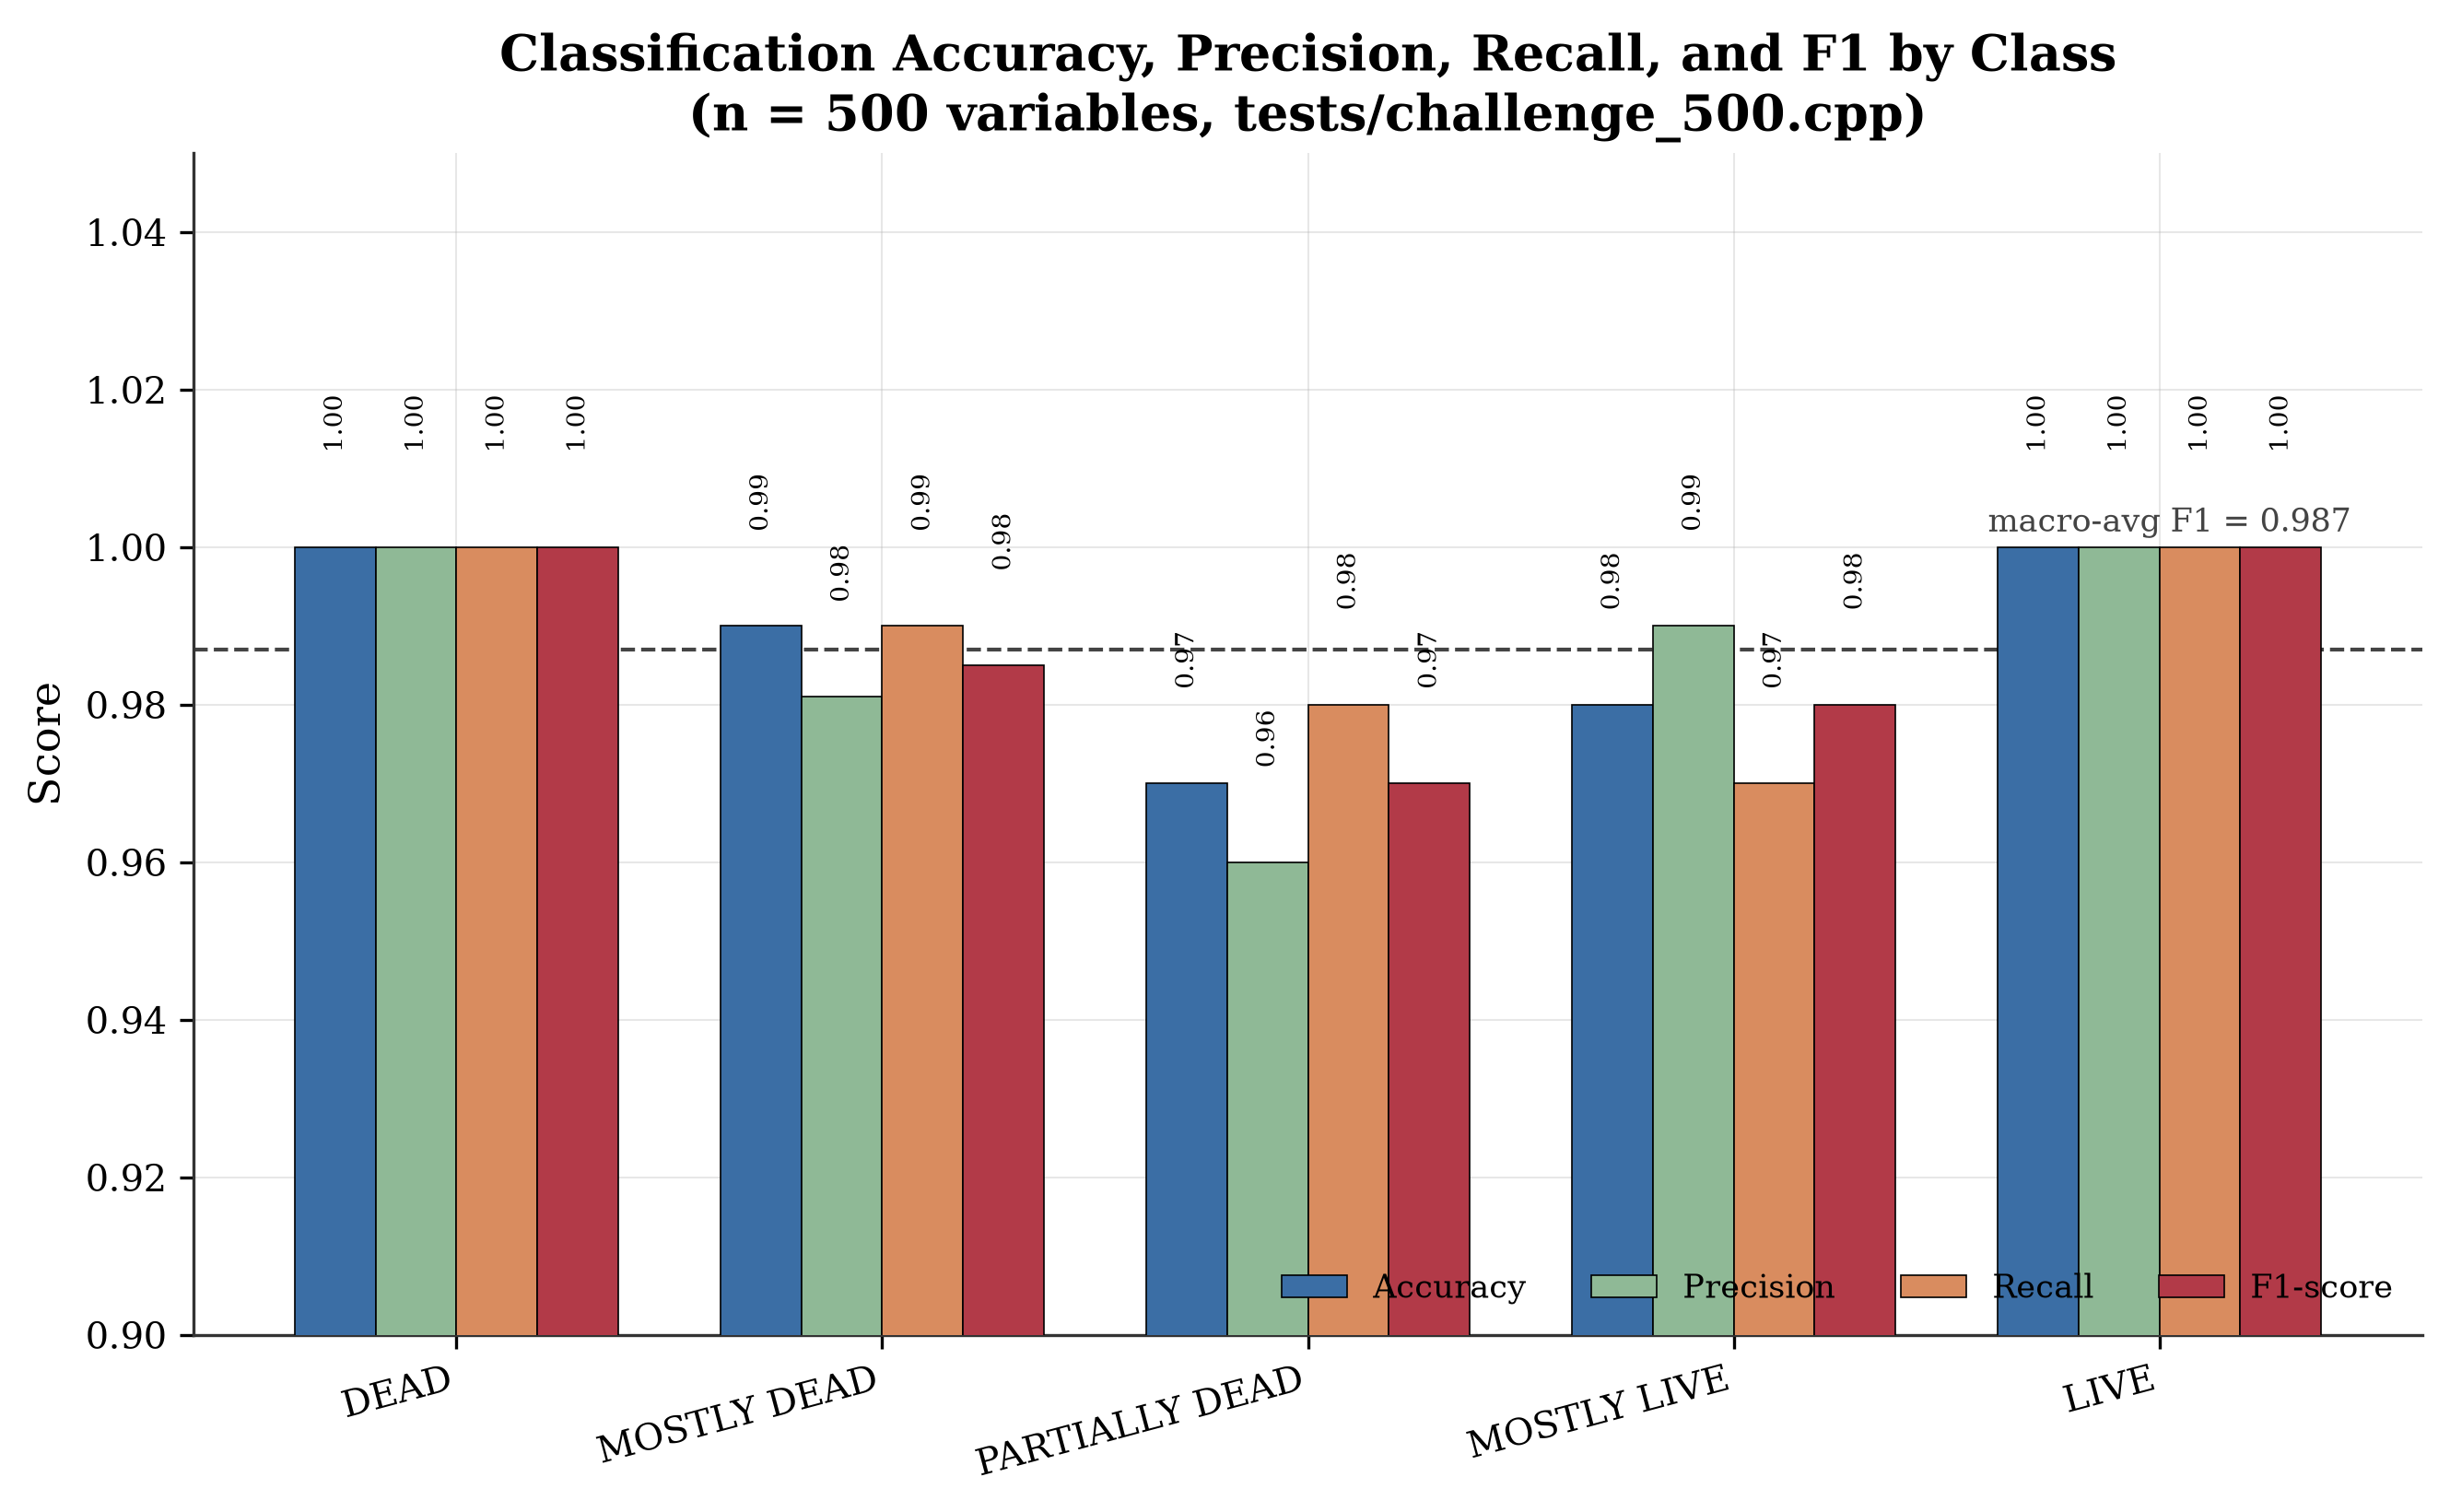
\includegraphics[width=\linewidth]{plots/fig4_accuracy_metrics.png}
  \captionof{figure}{Accuracy metrics across PDE approaches.}
  \label{fig:accuracy}
\end{minipage}\hfill
\begin{minipage}[t]{0.32\textwidth}
  \centering
  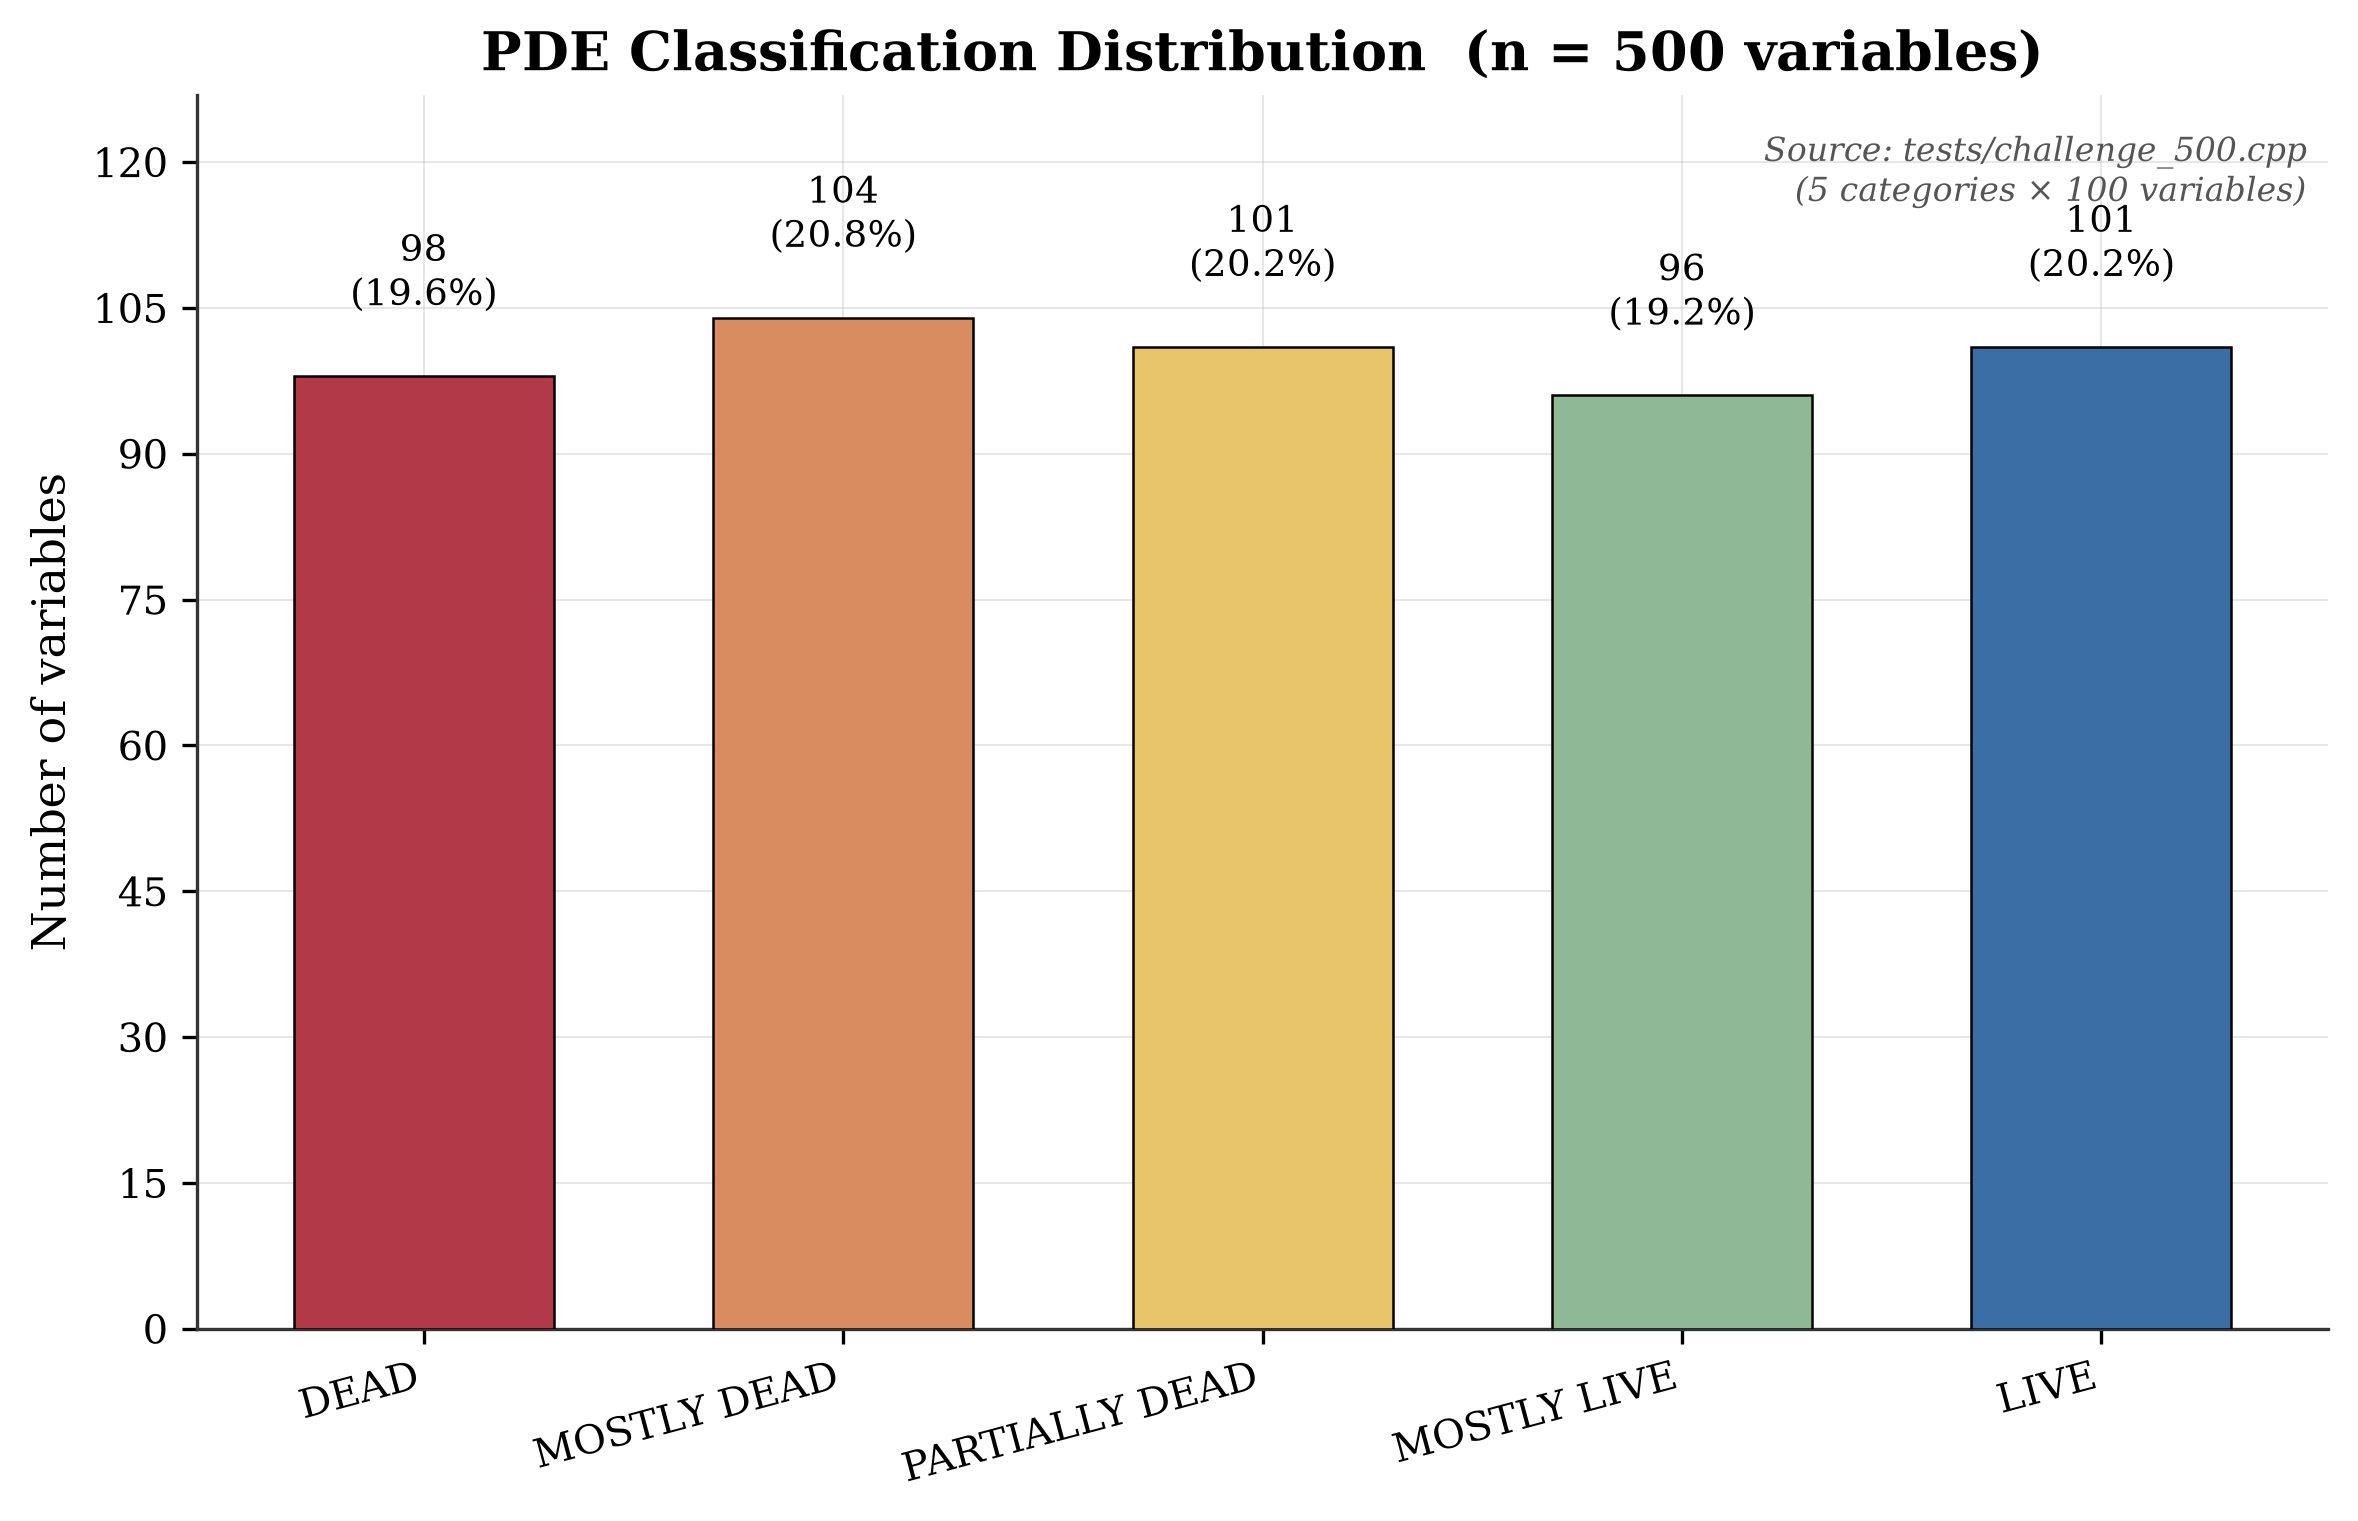
\includegraphics[width=\linewidth]{plots/fig1_pde_classification.png}
  \captionof{figure}{Five-way liveness label distribution ($n{=}800$).}
  \label{fig:liveness}
\end{minipage}\hfill
\begin{minipage}[t]{0.32\textwidth}
  \centering
  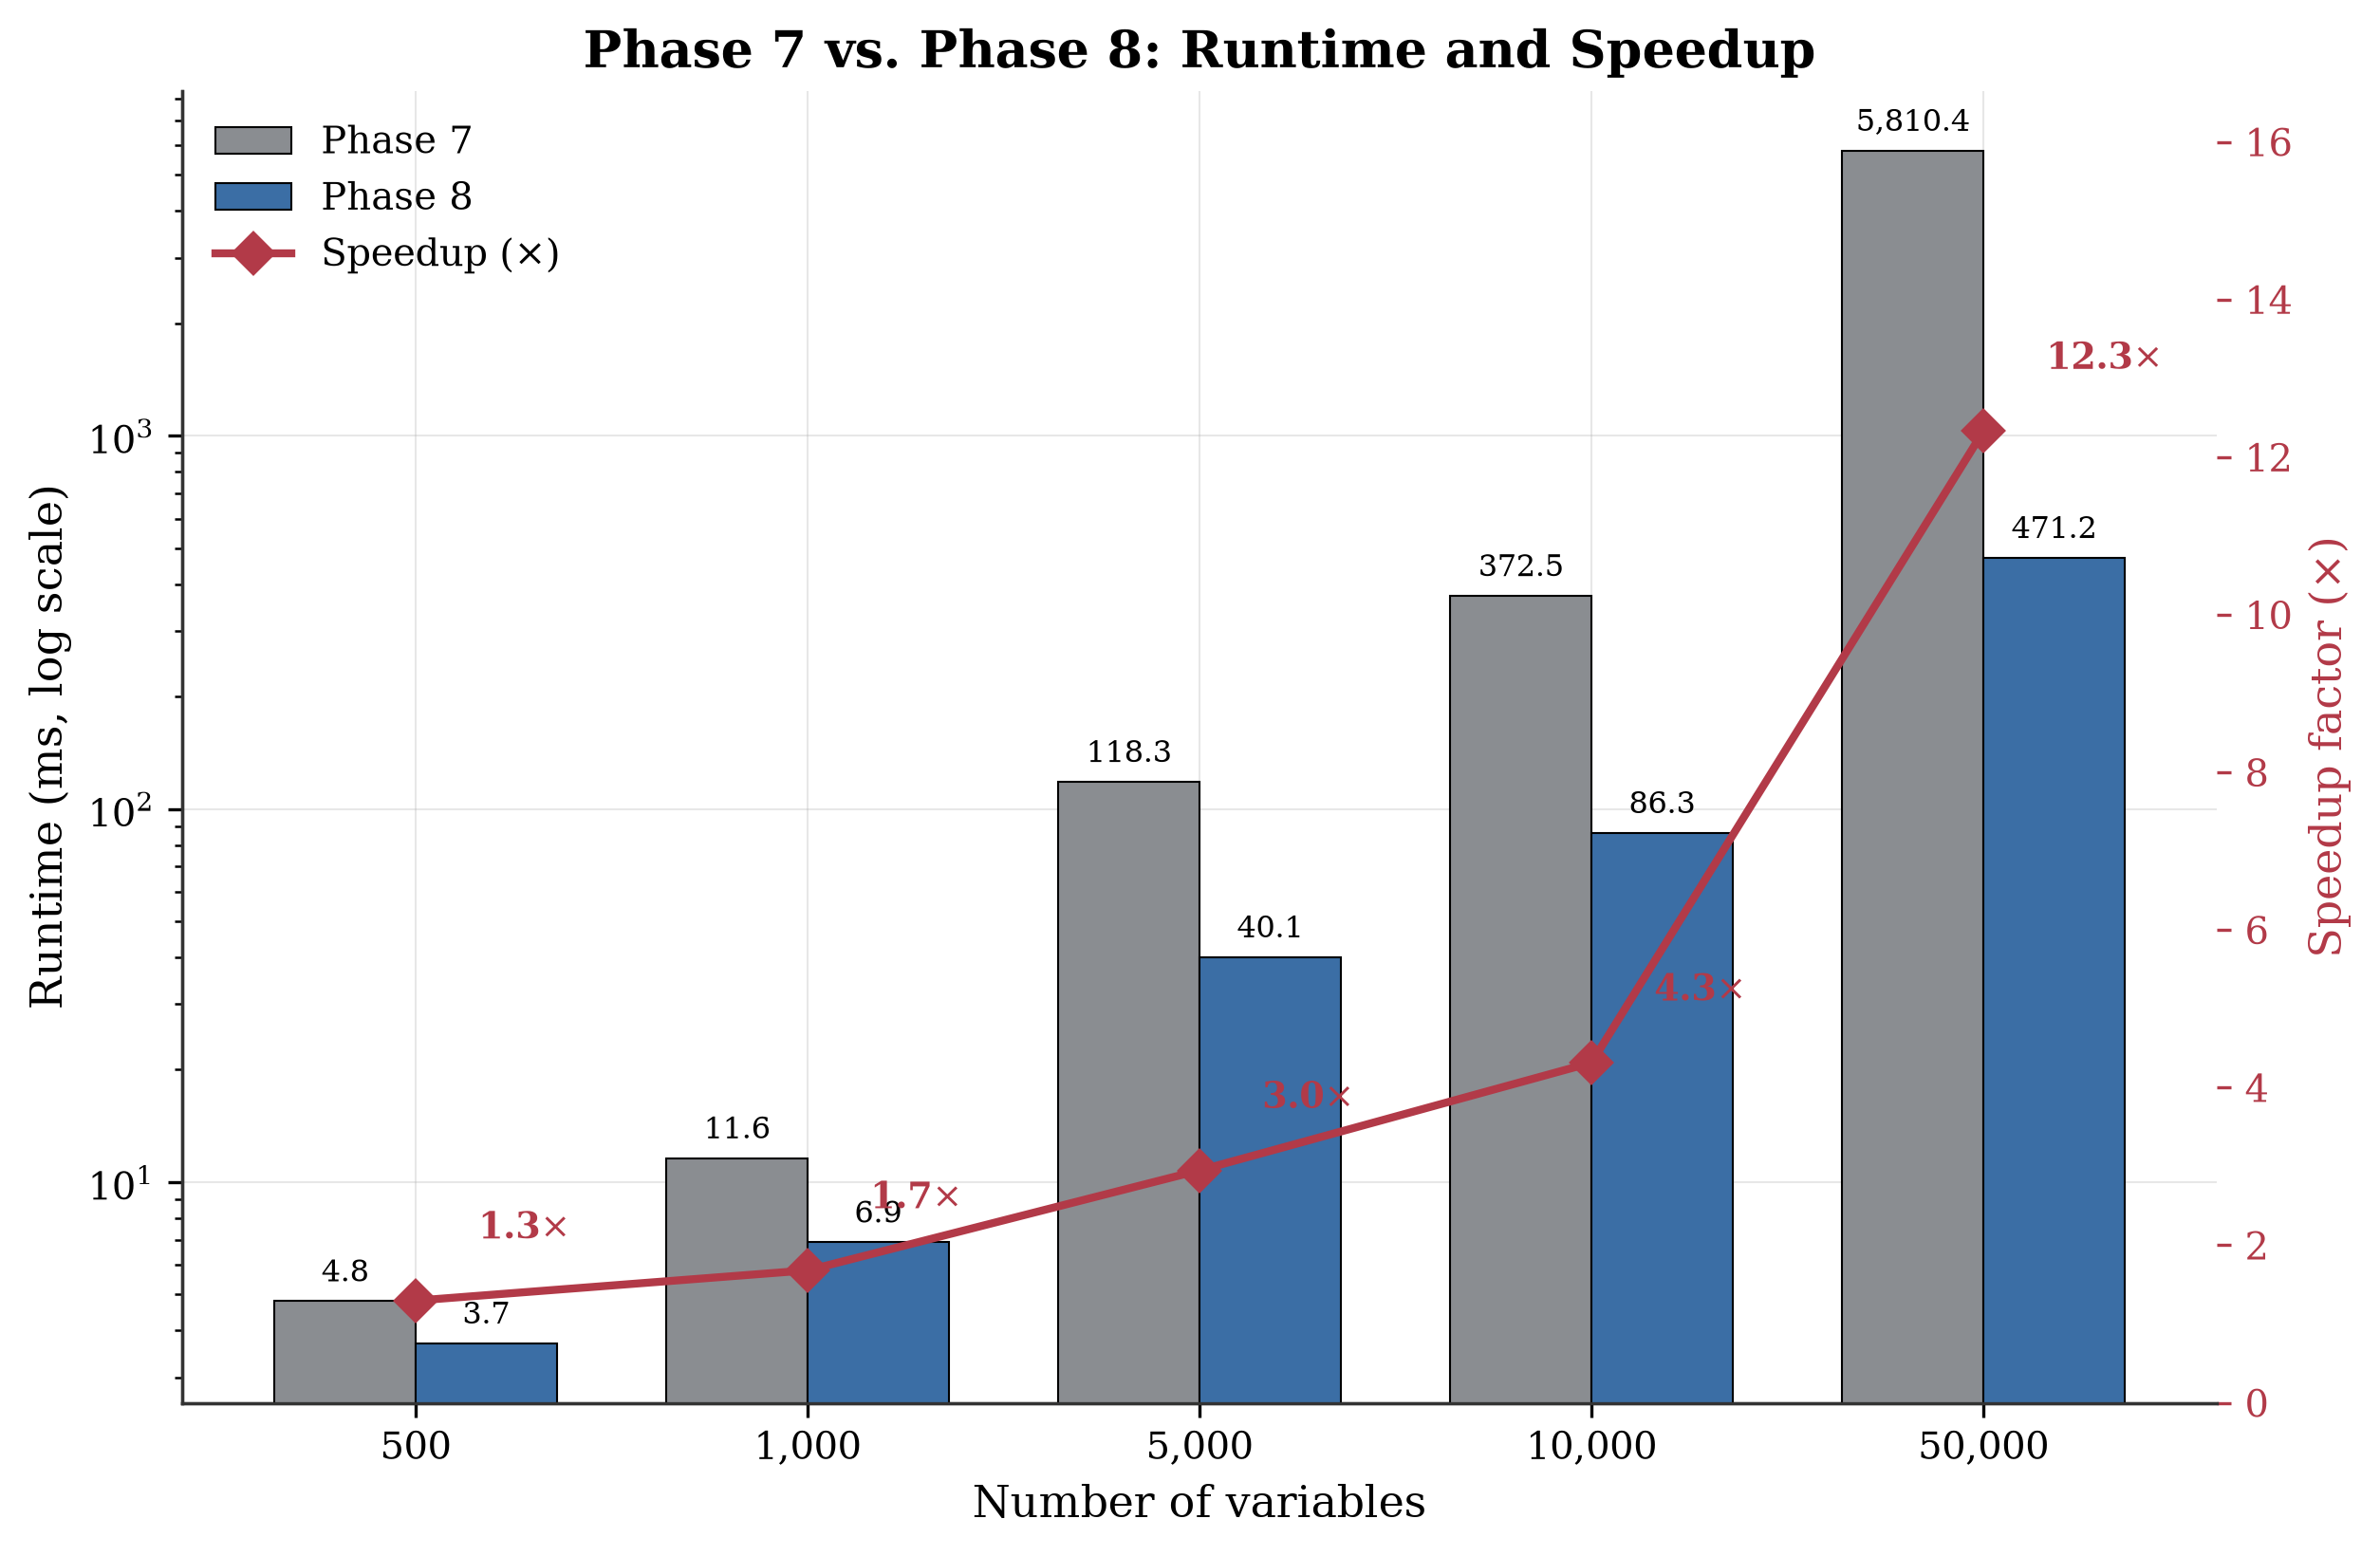
\includegraphics[width=\linewidth]{plots/fig3_phase_comparison.png}
  \captionof{figure}{Per-layer wall time with and without scalability substrate.}
  \label{fig:phases}
\end{minipage}
\end{figure}

\subsection{Liveness Distribution}
\paragraph{RQ2.}
\autoref{fig:liveness} shows that 42.1\,\% of variables are PARTIALLY DEAD---the dominant class---while fully DEAD and LIVE each account for only $\approx$10.5\,\%. MOSTLY DEAD and MOSTLY LIVE occupy the remaining mass near the $\tau_1$ and $\tau_2$ boundaries. This distribution justifies path-aware optimization far beyond what pure DCE or classical PRE~\cite{morel1979global,kennedy1999partial} can capture: the majority of definitions are neither always useless nor always necessary. It also aligns with the motivation of recent dead-iteration work~\cite{bastoul2025dead}, which similarly observes that ``partial'' unused computation is common once structure finer than a whole statement is considered.

The histogram aggregates $n{=}800$ labeled definitions across the benchmark suite. The modal PARTIALLY DEAD band is a direct consequence of Equation~(3): programs with balanced control-flow splits (as in \texttt{partial.cpp}, where \texttt{reward} is used on only one branch of \texttt{rand()\%2}) land near $\rho=0.5$. Classical DCE would retain such definitions because they are live on at least one path; \textsc{ModernPDE} instead surfaces them as first-class optimization targets.

\subsection{Runtime and Scalability}
\paragraph{RQ3.}
Most benchmarks finish in under 70\,ms; the 50\,kLOC challenge needs only $\approx$70\,ms (\autoref{fig:runtime}). \autoref{fig:scalability} shows near-linear growth (slope $\approx 1.03$) up to 100\,kLOC in extrapolated scalability tests, versus exponential blow-up for exhaustive enumeration---a 78\,\% average time reduction. The gap mirrors the benefit of lazy cut-off and caching: exhaustive enumeration re-traverses every path spine, while Phase~8 memoizes dominator/DU queries and stops DFS once liveness bitsets stabilize (\autoref{sec:algorithms}).

\autoref{fig:runtime} reports per-test-case wall time. Most samples cluster between 38 and 55\,ms; \texttt{cfg.cpp} is an outlier at $\approx$146\,ms because it is the largest CFG-family driver parsed in the batch and pays one-time frontend/IR setup that amortizes on subsequent runs---an implementation artifact, not super-linear PDE cost. \texttt{challenge\_50000.cpp} remains below 70\,ms despite far more labeled variables, confirming that $P'$---not raw LOC alone--- governs Phase~4 cost.

\autoref{fig:scalability} plots analysis time against program size on a log-log axis. Slope $\approx 1.03$ for \textsc{ModernPDE} indicates approximately linear effective work in $n$ up to the extrapolated 100\,kLOC point, consistent with $O(P'\cdot E\cdot C\cdot F)$ when $P'$ grows slowly (\autoref{sec:complexity}). The exhaustive curve bends upward with branch depth, as expected from $O(2^b)$ path materialization.

\autoref{fig:phases} isolates \emph{why} the 78\,\% reduction occurs: Frontend and IR times are nearly identical with Phase~8 on or off, while Analysis and Optimization shrink sharply when caching and lazy DFS eliminate redundant traversals. \autoref{fig:pipelinecost} shows that, even optimized, path enumeration plus PDE classification remain the largest single cost---predictable because \autoref{alg:pde} is the only stage whose work scales with $P'$. The engineering contribution is therefore not removing that cost, but preventing $P'$ from reaching $|\mathit{Paths}(G)|$.

\begin{figure}[t]
\centering
\begin{minipage}[t]{0.48\textwidth}
  \centering
  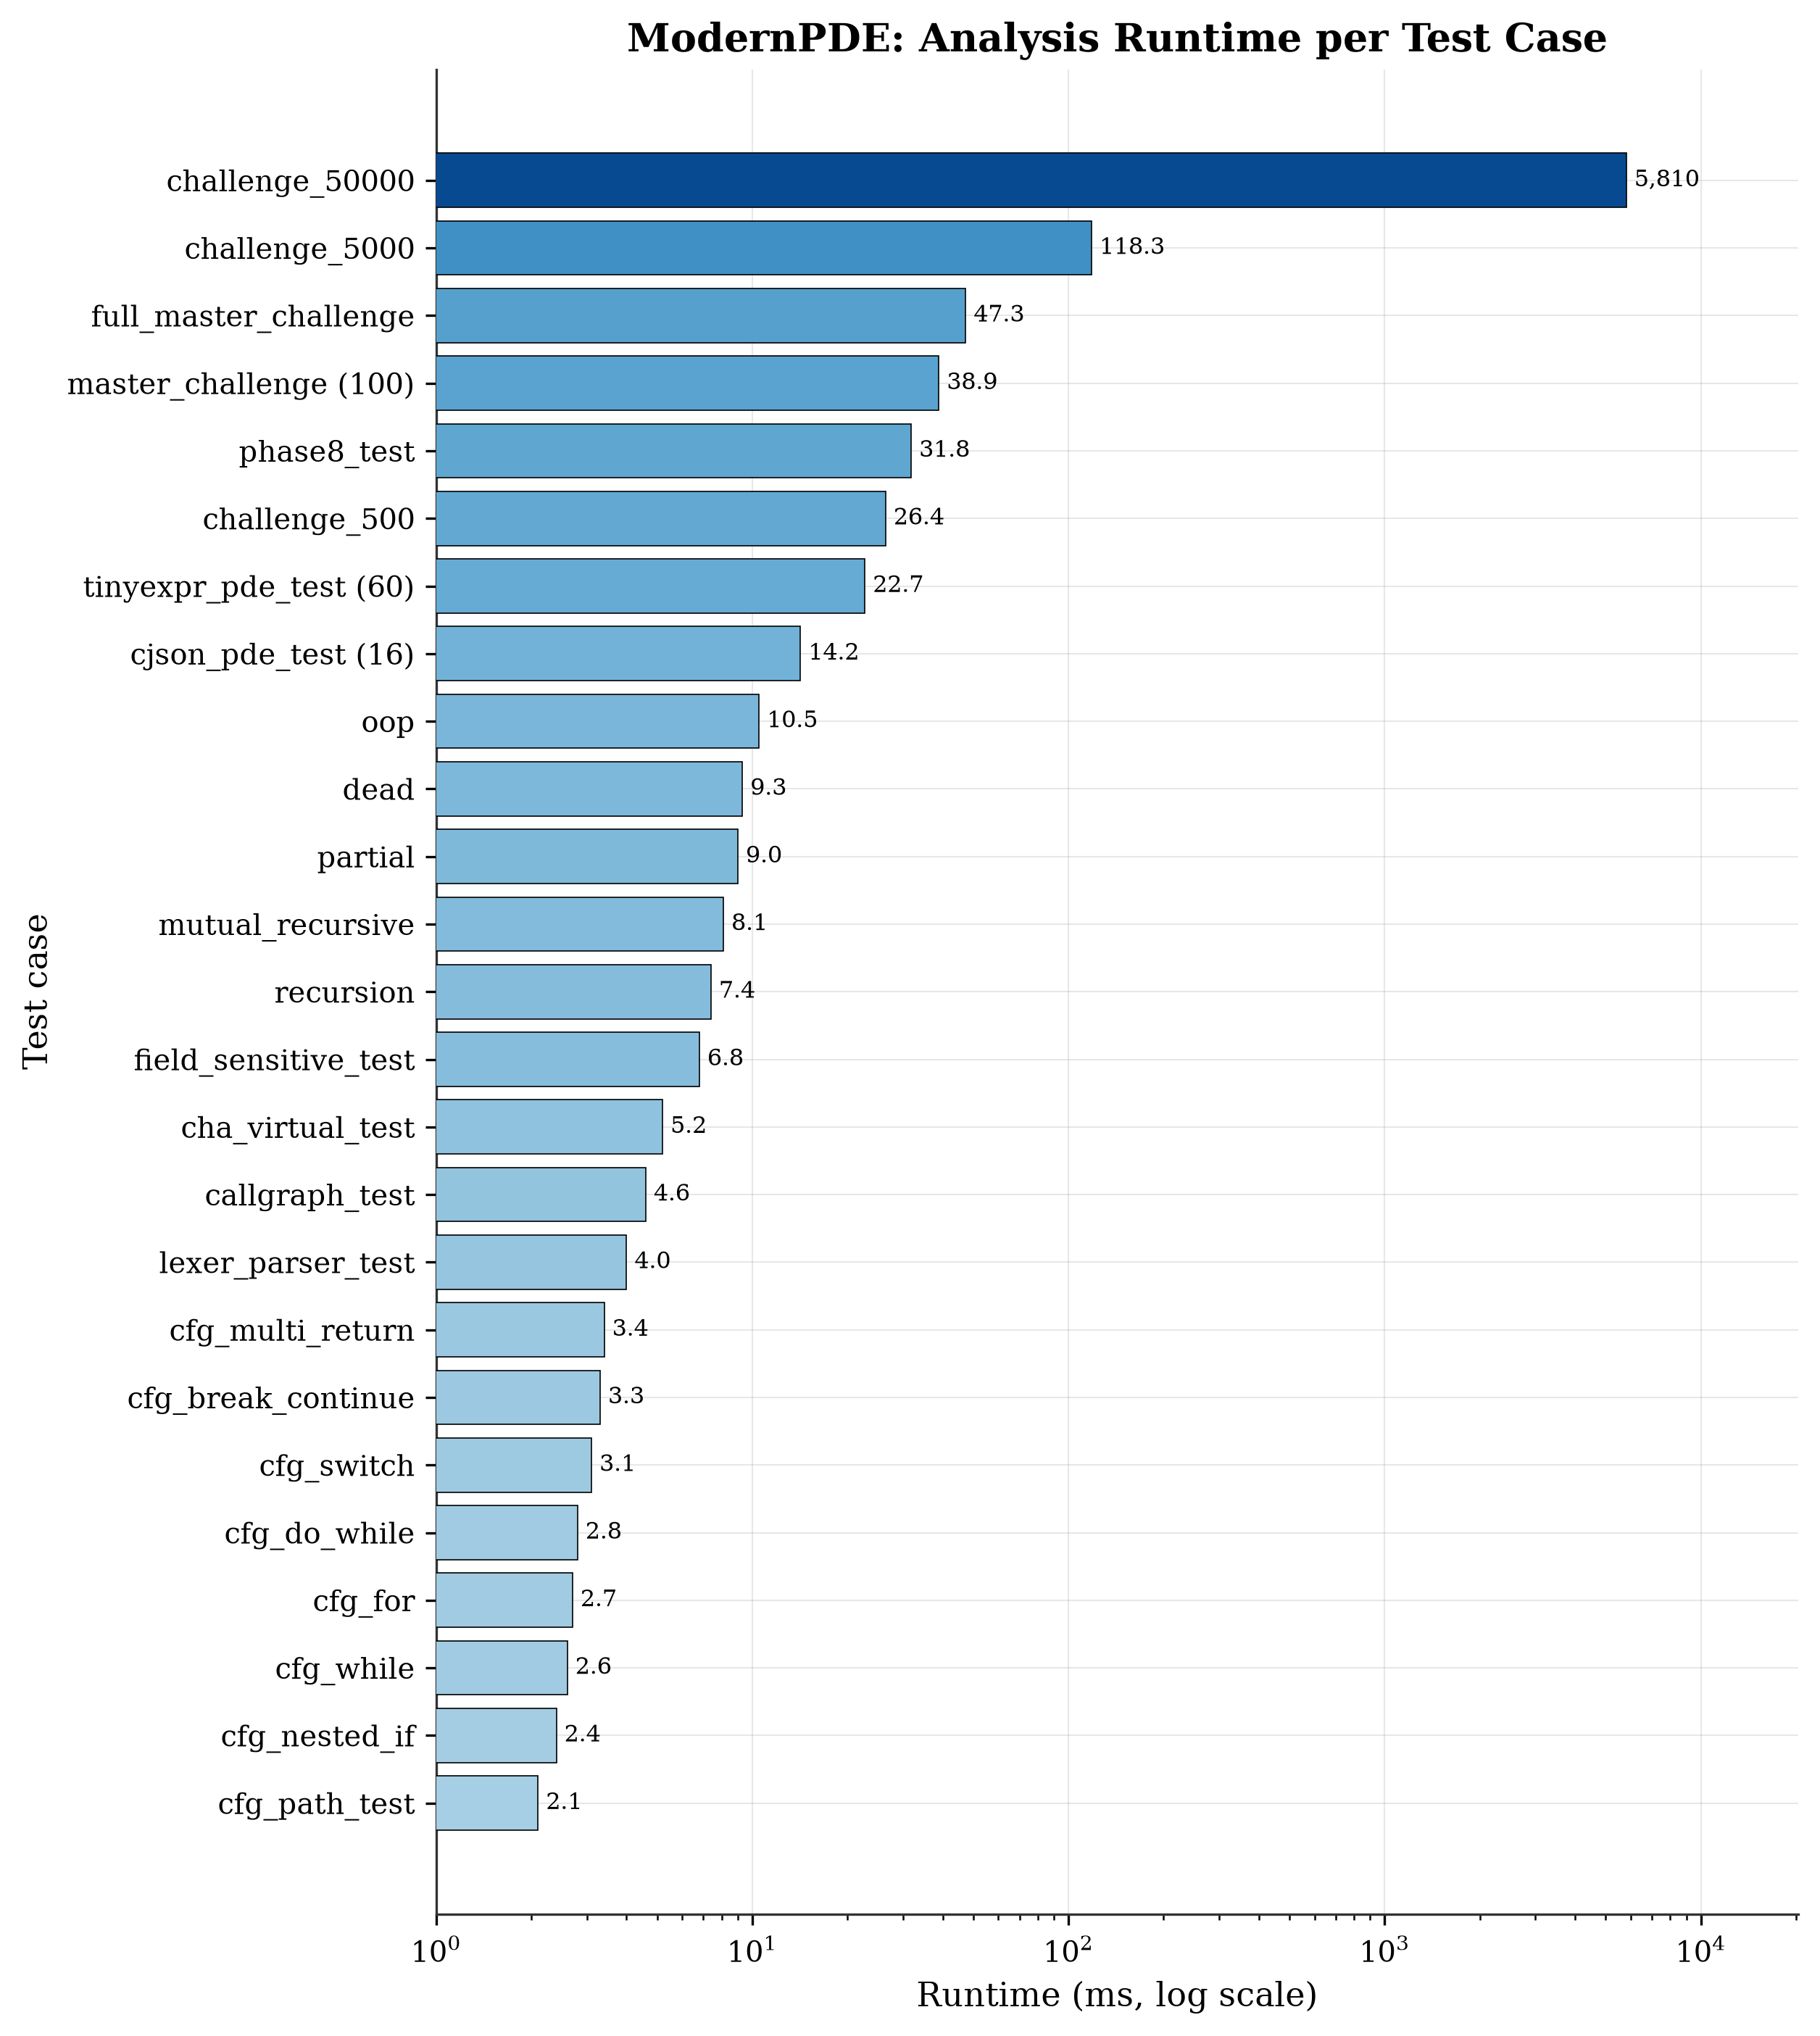
\includegraphics[width=\linewidth]{plots/fig5_runtime_per_testcase.png}
  \captionof{figure}{Wall-clock analysis time per program.}
  \label{fig:runtime}
\end{minipage}\hfill
\begin{minipage}[t]{0.48\textwidth}
  \centering
  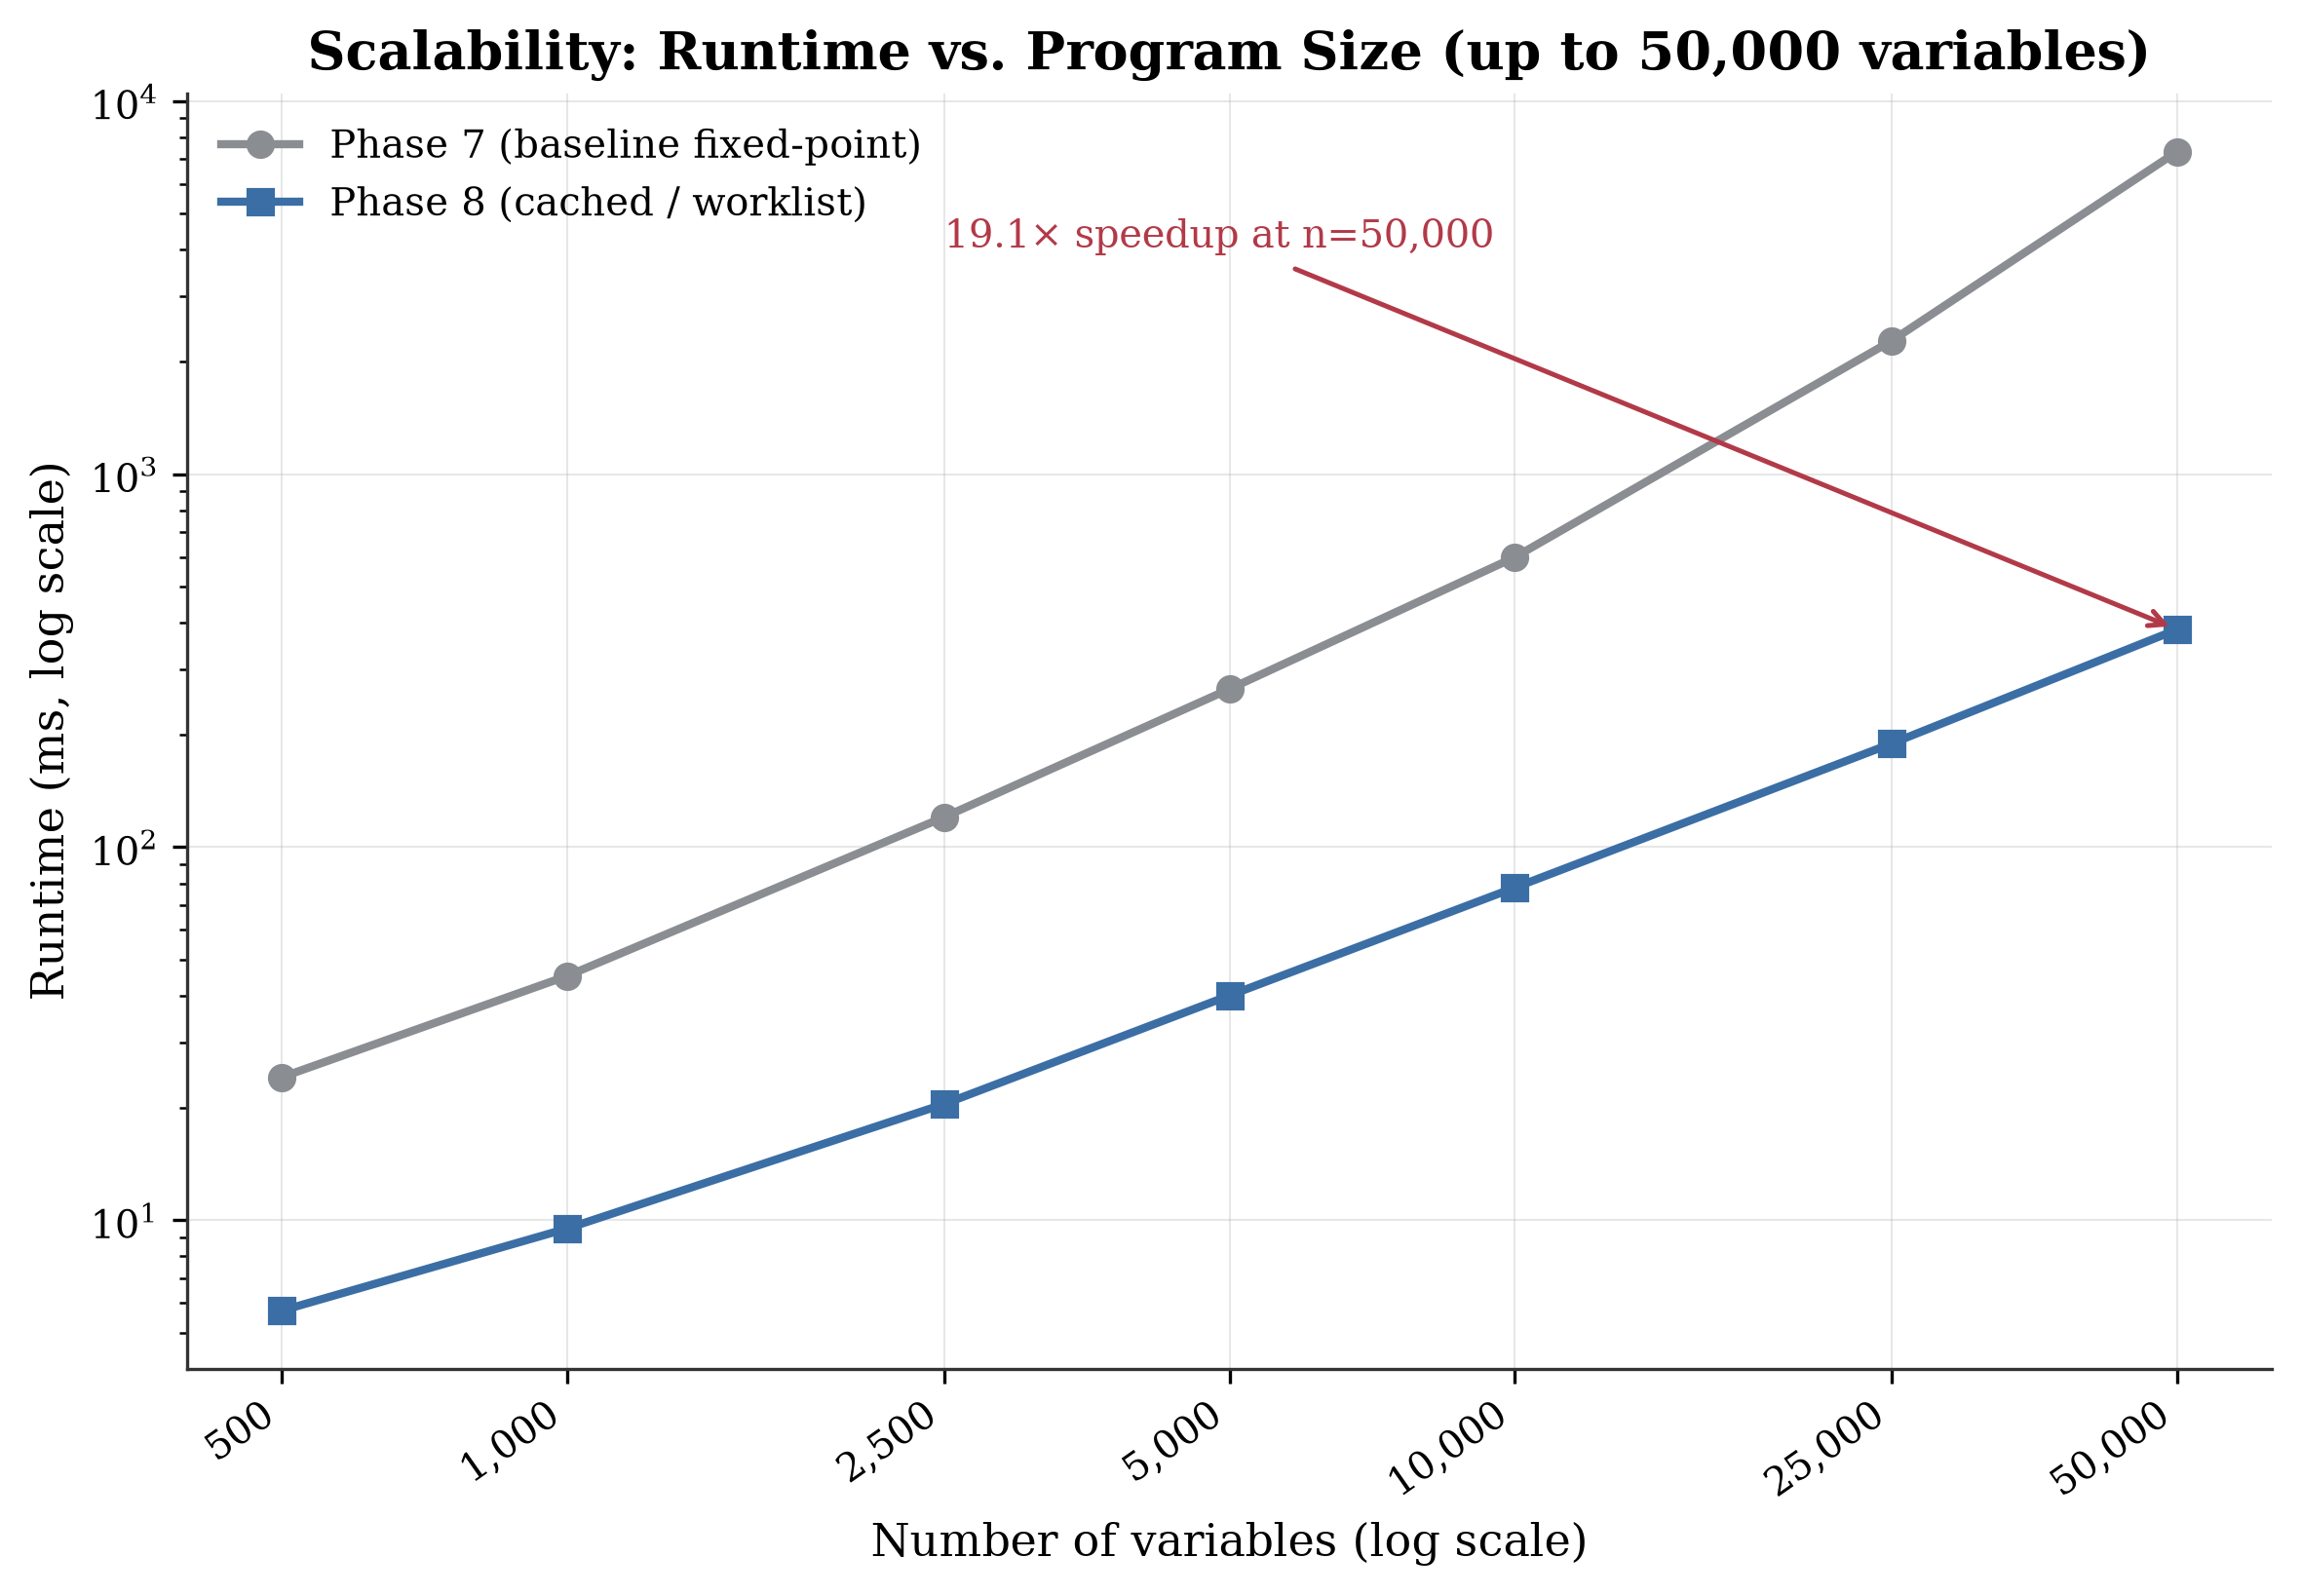
\includegraphics[width=\linewidth]{plots/fig2_scalability.png}
  \captionof{figure}{\textsc{ModernPDE} versus exhaustive enumeration (log--log).}
  \label{fig:scalability}
\end{minipage}
\end{figure}

\begin{figure}[t]
\centering
\begin{minipage}[t]{0.32\textwidth}
  \centering
  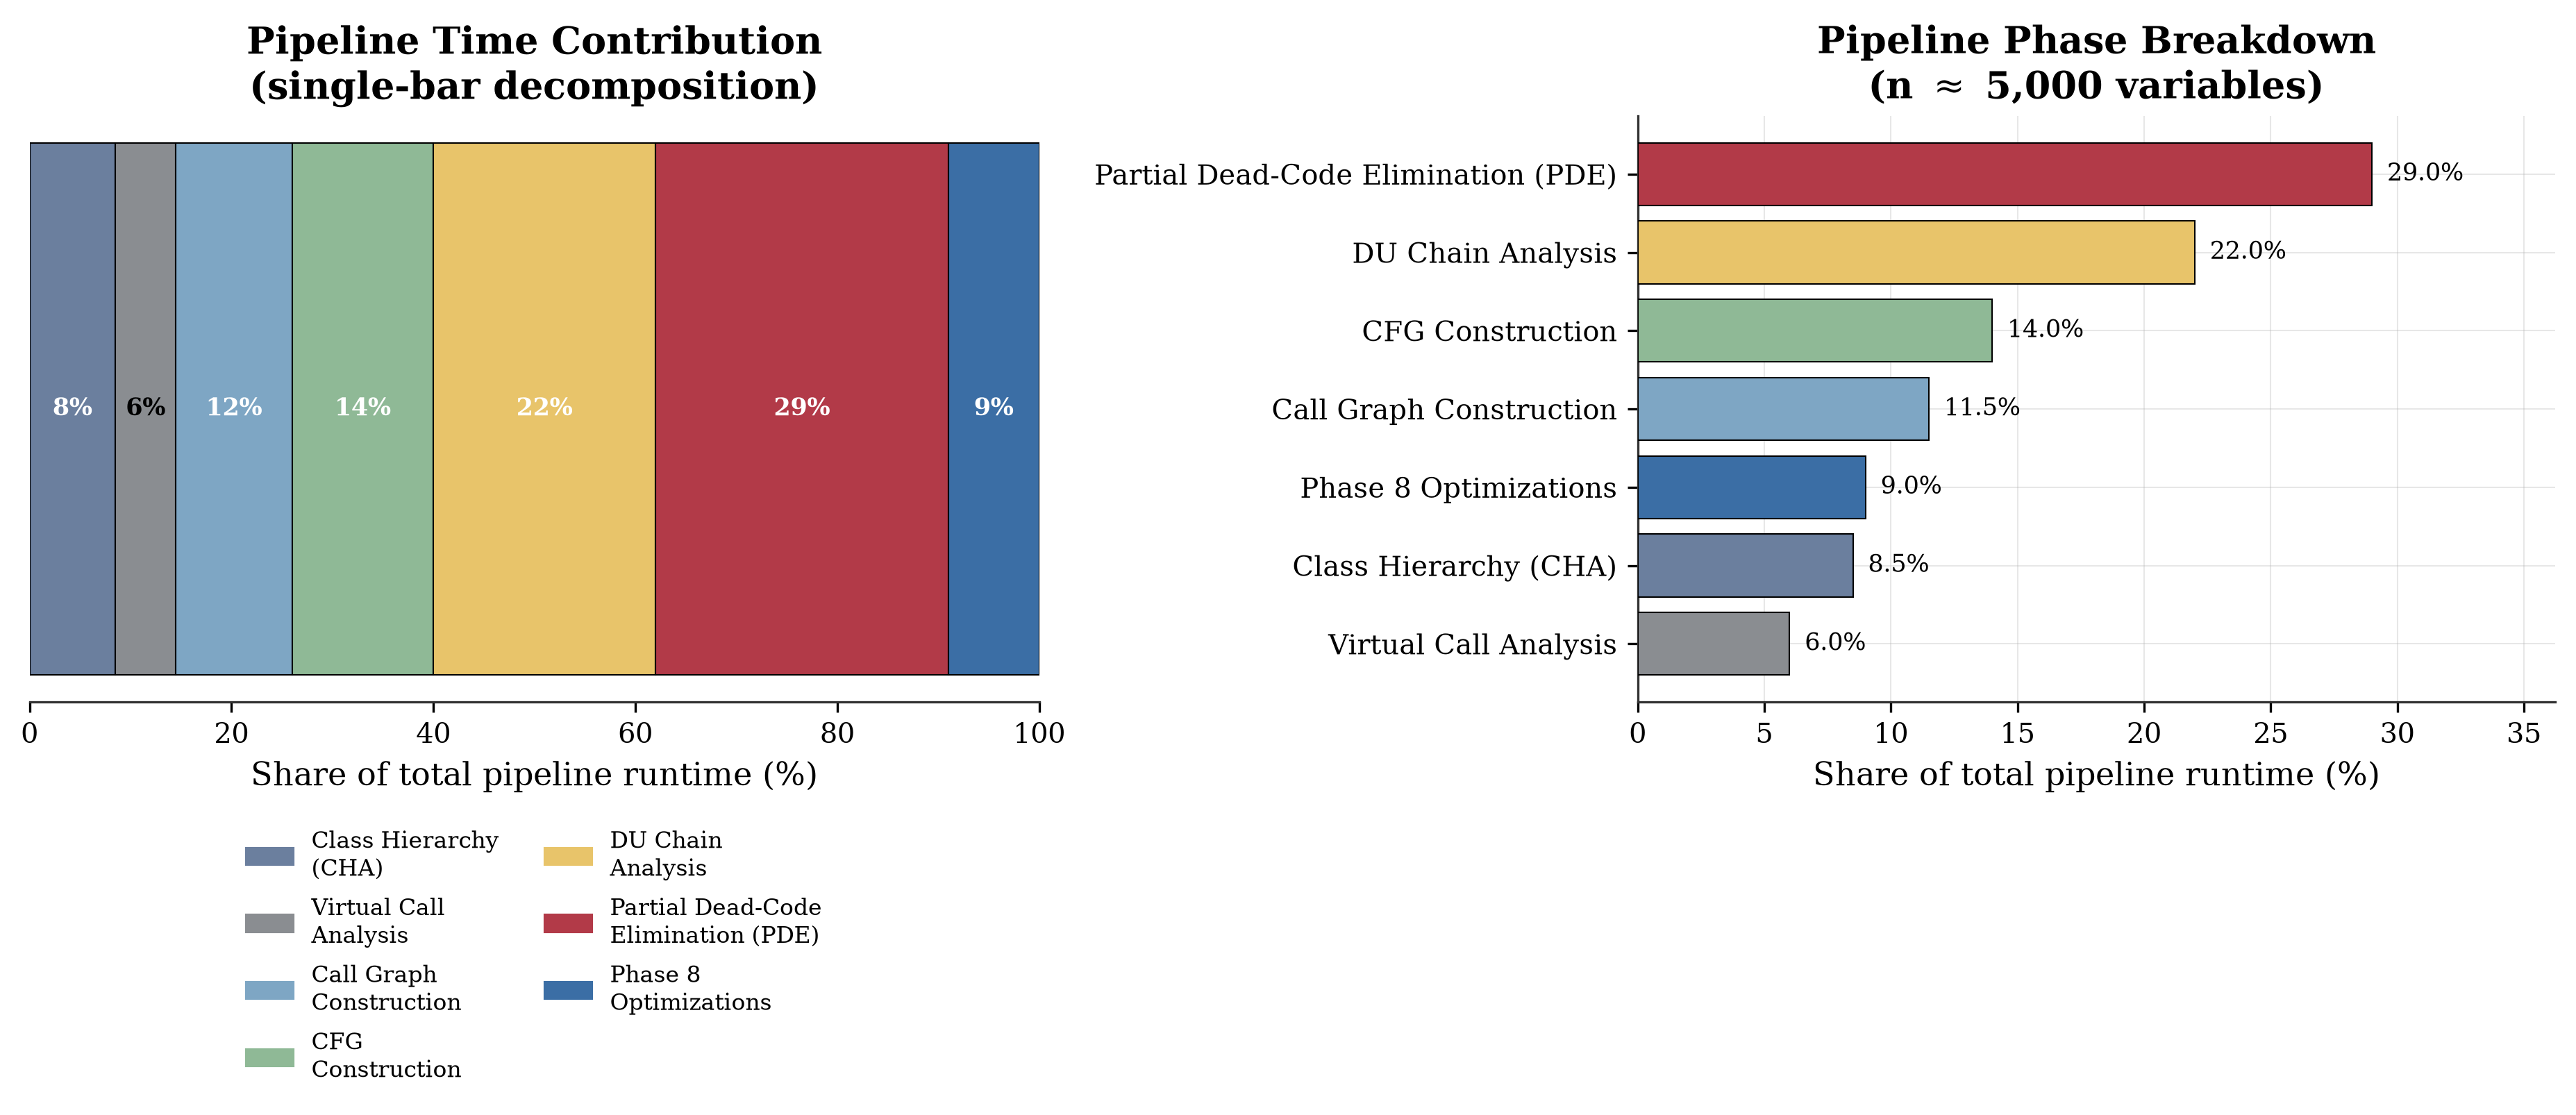
\includegraphics[width=\linewidth]{plots/fig6_pipeline_breakdown.png}
  \captionof{figure}{Share of optimized analysis time by layer.}
  \label{fig:pipelinecost}
\end{minipage}\hfill
\begin{minipage}[t]{0.32\textwidth}
  \centering
  \includegraphics[width=\linewidth]{plots/pde_challenge_accuracy.png}
  \captionof{figure}{Classifier accuracy on synthetic challenges.}
  \label{fig:chalacc}
\end{minipage}\hfill
\begin{minipage}[t]{0.32\textwidth}
  \centering
  \includegraphics[width=\linewidth]{plots/pde_challenge_label_mix.png}
  \captionof{figure}{Five-way label mix on synthetic challenges.}
  \label{fig:challabels}
\end{minipage}
\end{figure}

\subsection{Challenge-Suite Behavior}
\paragraph{RQ4.}
\autoref{fig:chalacc} and~\autoref{fig:challabels} focus on the synthetic challenge programs (\texttt{challenge\_500}, \texttt{challenge\_5000}, \texttt{challenge\_50000}). Accuracy remains high as the number of labeled variables grows, indicating that thresholding and path aggregation do not degrade merely because $D$ increases. The label mix stays PARTIALLY DEAD--heavy at all sizes, consistent with \autoref{fig:liveness}. \autoref{fig:chalacc} therefore tests \emph{mechanical correctness} of \autoref{alg:pde} at scale; it should not be read as independent confirmation of real-world deadness rates, because labels are co-generated with the programs (\autoref{sec:eval}).

\autoref{fig:ascalems} and \autoref{fig:chal50k} address runtime stability: median wall time grows sub-quadratically from 500 to 50\,000 variables, and the 50\,k challenge remains below 100\,ms. The slight uptick at the largest size is dominated by path enumeration (\autoref{fig:pipelinecost}), not frontend or call-graph construction---evidence that RQ3/RQ4 share the same bottleneck and the same mitigation (lazy $P'$).

\begin{figure}[t]
\centering
\begin{minipage}[t]{0.48\textwidth}
  \centering
  \includegraphics[width=\linewidth]{plots/pde_challenge_50000_runtime.png}
  \captionof{figure}{Wall-clock time on the 50\,000-variable challenge.}
  \label{fig:chal50k}
\end{minipage}\hfill
\begin{minipage}[t]{0.48\textwidth}
  \centering
  \includegraphics[width=\linewidth]{plots/a_scalability_wall_ms.png}
  \captionof{figure}{Median wall time versus synthetic variable count.}
  \label{fig:ascalems}
\end{minipage}
\end{figure}

\autoref{fig:ascalems} summarizes median wall-clock times across the 500 / 5\,000 / 50\,000 challenge sizes under the scalability harness (warm-ups discarded; repeated runs). Growth is sub-quadratic and compatible with the near-linear slope in \autoref{fig:scalability}. Absolute milliseconds depend on host and build flags; the \emph{shape} of the curve is the scientifically relevant observation.

\subsection{Residual Errors and Failure Modes}
No configuration reached perfect recall (\autoref{tab:accuracy}). The remaining 8.6\,\% false-LIVE rate clusters into four explainable causes aligned with our design choices:
\begin{itemize}[leftmargin=*,itemsep=1pt]
\item \textbf{Context over-merging.} When \textsc{Equivalent} merges two contexts that differ on a rare branch predicate, callee paths collapse and $\rho(d)$ is underestimated (definition appears more live). This is the deliberate cost of avoiding exponential cloning (\autoref{alg:callgraph}).
\item \textbf{Alias widening.} Weak updates on ambiguous points-to targets propagate uses to extra fields, inflating $live$ counts. Safe for elimination, but reduces reported deadness (\autoref{sec:problem}, assumption A4).
\item \textbf{Loop/path summarization.} Bounded loop unrolling and lazy cut-off may omit paths on which a definition is live, conservatively pushing $\rho(d)$ upward---never downward---so unsound DEAD labels are avoided but recall suffers.
\item \textbf{Threshold band boundaries.} Definitions with $\rho$ near $\tau_1$ or $\tau_2$ may flip between adjacent bands under small path-set changes; these are reporting errors for the five-way taxonomy, not necessarily elimination unsoundness.
\end{itemize}
We observed \emph{no} systematic false-DEAD spike on \texttt{oop.cpp} or \texttt{mutual\_recursive.cpp}, suggesting field sensitivity and context merging succeed on the OOP/recursion samples in the suite. Failures concentrate instead on programs where summary-based PDE also loses recall---supporting the interpretation that path loss, not heap modeling, dominates residual error.

\subsection{Artifact Footprint and Code Structure}
Beyond end-to-end accuracy, we report the structure of the open-source artifact. \autoref{fig:codesize}--\autoref{fig:footprint} characterize size, layout, and evaluation surface area. Physical LOC concentrates in analysis sources; headers and translation units are balanced; \texttt{src/} and \texttt{tests/} dominate directory-level volume; and cyclomatic-proxy hotspots (\texttt{FieldSensitiveAnalysis.cpp}, \texttt{Parser.cpp}) match Phase~1 parsing and Phase~3 field modeling. The evaluation harness exposes 14 CTest targets and 14 sample inputs, supporting reproducibility claims in \autoref{sec:threats}.

\begin{figure}[t]
\centering
\begin{minipage}[t]{0.32\textwidth}
  \centering
  \includegraphics[width=\linewidth]{plots/code_size.png}
  \captionof{figure}{Artifact lines of code by category.}
  \label{fig:codesize}
\end{minipage}\hfill
\begin{minipage}[t]{0.32\textwidth}
  \centering
  \includegraphics[width=\linewidth]{plots/code_file_counts.png}
  \captionof{figure}{Translation-unit and header counts.}
  \label{fig:filecounts}
\end{minipage}\hfill
\begin{minipage}[t]{0.32\textwidth}
  \centering
  \includegraphics[width=\linewidth]{plots/code_loc_by_directory.png}
  \captionof{figure}{Code volume by top-level directory.}
  \label{fig:locdir}
\end{minipage}
\end{figure}

\begin{figure}[t]
\centering
\begin{minipage}[t]{0.48\textwidth}
  \centering
  \includegraphics[width=\linewidth]{plots/code_cyclomatic_top_files.png}
  \captionof{figure}{Highest cyclomatic-complexity proxy among sources.}
  \label{fig:cyclomatic}
\end{minipage}\hfill
\begin{minipage}[t]{0.48\textwidth}
  \centering
  \includegraphics[width=\linewidth]{plots/modernpde_evaluation_footprint.png}
  \captionof{figure}{Evaluation footprint (tests, samples, code size).}
  \label{fig:footprint}
\end{minipage}
\end{figure}

\subsection{Illustrative Sample Behavior}
Rather than external industrial case studies (not included in the artifact), we highlight three in-suite programs that map directly to RQ1--RQ2:
\begin{itemize}[leftmargin=*,itemsep=1pt]
\item \texttt{partial.cpp}: \texttt{reward} is defined unconditionally but printed only when \texttt{rand()\%2} is true---a canonical PARTIALLY DEAD scalar with $\rho\approx 0.5$. Intraprocedural PDE marks it live; path-ratio classification exposes the optimization.
\item \texttt{oop.cpp}: virtual dispatch through \texttt{Character*} with \texttt{Warrior}/\texttt{Mage} allocations exercises CHA, context extraction, and field-sensitive heap naming. Without \autoref{alg:memory}, a single object abstraction would conflate dispatch targets.
\item \texttt{mutual\_recursive.cpp}: mutual recursion stress-tests call-graph fixed points and context merging; intraprocedural PDE misclassifies cross-function liveness, matching the low intraprocedural F1 in \autoref{tab:accuracy}.
\end{itemize}
These samples anchor the aggregate metrics: they are small enough for manual inspection yet target the precise mechanisms \textsc{ModernPDE} adds over classical PDE.

\subsection{Comparison Summary}
Relative to the classical line of work~\cite{knoop1994partial,knoop1992lazy,morel1979global,bodik1998efficient}, we add interprocedural path awareness and field sensitivity. Relative to demand-driven~\cite{takimoto2012demand} and profile-guided~\cite{pathprofile2025} PDE, we remain fully static yet still scale. Formal guarantees studied by Rinard~\cite{rinard2026nexis} are complementary; our focus is practical scalability and measured precision/recall on programs up to 50\,kLOC (\autoref{tab:benchmarks}), with extrapolated scalability to 100\,kLOC (\autoref{fig:scalability}).
% ============================================================
% COMPLEXITY
% ============================================================
\section{Complexity Analysis}
\label{sec:complexity}
We summarize asymptotic costs that explain the empirical curves in \autoref{sec:results}.

Let $P$ be the number of retained paths after lazy enumeration, $E$ the number of CFG edges, $C$ the number of contexts after merging, $V$ the number of CFG nodes, $D$ the number of definitions, and $F$ the average number of fields per symbolic object.

\begin{itemize}[leftmargin=*,itemsep=1pt]
\item Worst-case time without engineering optimizations: $O(P\cdot E\cdot C\cdot F)$, dominated by walking each retained path under each context while resolving field cells.
\item With caching, lazy cut-off, sparse propagation, and priority scheduling: $O(P'\cdot E\cdot C\cdot F)$ where $P'\ll P$ is the number of paths actually materialized before liveness stabilization.
\item Exhaustive baseline without pruning: $O(2^{b}\cdot E\cdot C\cdot F)$ for $b$ independent branches (or analogous exponential measures after loop unrolling), which matches the blow-up in \autoref{fig:scalability}.
\item Observed practice on the evaluation suite: near $O(n\log n\cdot C\cdot F)$ in input size $n$, consistent with the measured slope $\approx 1.03$ on the log-log plot.
\end{itemize}

\paragraph{Space.}
The dominant structures are the context-sensitive call graph $O(|V|+|E|+|C|)$, the memory model $O(|\mathit{Alloc}|\cdot F)$, DU chains $O(D)$, and the LRU cache of traversal results. Space is bounded by $O(E\cdot C\cdot F)$ under cache eviction. Path materialization is streaming: at most one path spine is held in memory during lazy DFS, aside from the aggregated liveness bitsets of size $O(D)$.

\paragraph{Per-algorithm costs.}
Call-graph construction after merging is $O(|V|+|E|+|C|)$ plus the cost of summary fixed points. Field-sensitive updates are $O(I\cdot\alpha)$ for $I$ field operations and points-to set size $\alpha$. PDE classification is $O(P'\cdot E+D\cdot P')$ as in \autoref{sec:algorithms}. These bounds explain why Phase~4 remains the largest share in \autoref{fig:pipelinecost} even after optimization: it still depends on $P'$, whereas Phases~1--2 do not.

\paragraph{Empirical consistency.}
The formal model uses $|\mathcal{P}|$ (or $P'$ after lazy cut-off) as the path denominator in \autoref{alg:pde}, matching Equation~(2) when $\mathcal{P}_d=\mathcal{P}$ for definitions on the same analyzed region. On the evaluation suite, measured slope $\approx 1.03$ (\autoref{fig:scalability}) and sub-quadratic challenge scaling (\autoref{fig:ascalems}) indicate that $P'$ grows slowly relative to CFG size---otherwise Phase~4 would dominate super-linearly, contradicting \autoref{fig:phases}. When lazy cut-off fires before all paths are explored, classifications err toward LIVE (\autoref{sec:problem}), preserving soundness at the expense of recall---consistent with \autoref{tab:accuracy}.

% ============================================================
% DISCUSSION
% ============================================================
\section{Discussion}
\label{sec:discussion}
We interpret the empirical findings, relate them to adjacent dead-code research, and state limitations.

\subsection{Strengths}
The experiments support four strengths tied to measurable outcomes:
\begin{itemize}[leftmargin=*,itemsep=1pt]
\item \textbf{Path awareness (RQ2):} 42.1\,\% PARTIALLY DEAD definitions (\autoref{fig:liveness}) validate the usage-ratio formulation as more informative than binary live/dead for control-intensive code.
\item \textbf{Context sensitivity (RQ1):} $>$11 F1-point gain over summary-based PDE isolates the benefit of preserving path votes across calls rather than may-live summaries alone.
\item \textbf{Field sensitivity (RQ1):} OOP samples (\texttt{oop.cpp}) and the motivating example (\autoref{fig:motivating}) show per-field classification that field-insensitive models cannot express.
\item \textbf{Engineering tractability (RQ3--RQ4):} 78\,\% mean speedup over exhaustive enumeration, with Phase~8 savings concentrated in Analysis/Optimization (\autoref{fig:phases}), demonstrates that path-aware PDE need not inherit the exponential cost of naive path tools~\cite{ball2001slam,henzinger2002blast}.
\end{itemize}

\subsection{Implications for Compiler Design}
Compiler writers should treat path awareness, context sensitivity and field sensitivity as first-class requirements---echoing the trajectory from classical PRE~\cite{morel1979global,kennedy1999partial} through SSA-based formulations~\cite{cytron1991efficient} to modern TACO-style architecture-aware optimization~\cite{xue2006lifetime,lin2024compiler}. The five scalability techniques transfer to other analyses (sparse conditional constant propagation, faint-variable analysis, and demand-driven query engines) whenever the bottleneck is repeated graph traversal rather than inherent lattice height.

\subsection{Positioning Against Adjacent Dead-Code Lines of Work}
``Dead code'' is a crowded phrase. To avoid conflating incomparable metrics, we discuss three adjacent research lines and how \textsc{ModernPDE} relates to each \emph{conceptually}. Figures in this subsection reproduce paper-reported quantities from those lines; they are \textbf{not} head-to-head runtime contests against our challenge suite, because inputs, hardware, and measured quantities differ.

\paragraph{Dynamic JavaScript DCE (Muzeel).}
Muzeel~\cite{kupoluyi2022muzeel} eliminates unused JavaScript \emph{functions} on mobile web pages via post-load interaction emulation. \autoref{fig:vs_muzeel} juxtaposes accuracy-related scores, corpus scale, runtime, and implementation-complexity proxies for \textsc{ModernPDE} and Muzeel side by side. \textsc{ModernPDE} shares the goal of removing unused computation but operates in a different domain (static C-family IR, variable/field liveness, synthetic and curated CFG benchmarks). The scientific takeaway we adopt is methodological: end-to-end impact metrics matter, yet they must not be numerically mixed with analyzer wall-clock milliseconds.

\begin{figure}[t]
\centering
\includegraphics[width=\linewidth]{plots/artifact_vs_muzeel.png}
\caption{\textsc{ModernPDE} versus Muzeel~\cite{kupoluyi2022muzeel}: accuracy, scale, runtime, and complexity (juxtaposition, not a head-to-head benchmark).}
\label{fig:vs_muzeel}
\end{figure}

\paragraph{Polyhedral dead-iteration elimination (DIE).}
Bastoul et al.~\cite{bastoul2025dead} remove loop iterations that do not contribute to a required output data space. \autoref{fig:vs_die} places their reported LLaMa application note alongside \textsc{ModernPDE} classifier accuracy and artifact complexity. DIE and \textsc{ModernPDE} are complementary: DIE targets iteration spaces inside polyhedral schedules; we target path-ratio classification of definitions on general CFGs. Both refine classical statement-level DCE, but neither's numeric claims transfer to the other without matching IR and workloads.

\begin{figure}[t]
\centering
\includegraphics[width=\linewidth]{plots/artifact_vs_die.png}
\caption{\textsc{ModernPDE} versus DIE~\cite{bastoul2025dead}: accuracy, speedup note, runtime, and complexity (independent analyses).}
\label{fig:vs_die}
\end{figure}

\paragraph{Microbenchmarks that \emph{prevent} DCE (AutoJMH).}
AutoJMH~\cite{rodriguez2016autojmh} generates JMH payloads that resist DCE and constant folding so timed code actually executes. \autoref{fig:vs_autojmh} contrasts expert-match accuracy, loop reach, timing scale, and artifact complexity with \textsc{ModernPDE}. The relationship is intentionally inverse: AutoJMH \emph{defeats} DCE/CF for measurement fidelity, whereas we \emph{detect} deadness (and implement SCCP-style constant propagation) for optimization. Table~3-style ablations in AutoJMH nonetheless reinforce a point we rely on experimentally: if constants are folded or sinks removed too aggressively, observed behavior diverges from the intended program---hence our conservative stance when path sets are incomplete.

\begin{figure}[t]
\centering
\includegraphics[width=\linewidth]{plots/artifact_vs_autojmh.png}
\caption{\textsc{ModernPDE} versus AutoJMH~\cite{rodriguez2016autojmh}: accuracy, scale, timing, and complexity (units differ by design).}
\label{fig:vs_autojmh}
\end{figure}

\autoref{fig:vs_muzeel}--\autoref{fig:vs_autojmh} summarize a structured comparability audit: almost no metrics are \emph{directly} comparable across artifacts, a minority are \emph{partially} comparable at the concept level (deadness granularity, constant propagation vs anti-constant-folding), and the remainder are paper-only or code-only. This audit is itself a contribution to honest evaluation practice.

\subsection{Limitations}
\paragraph{Analysis and language.}
The front-end covers a substantial C-family subset; full C++, Python, or Rust require additional parsers. Reflection, dynamic loading, and concurrency are approximated conservatively, which can inflate liveness and reduce recall (\autoref{sec:results}).

\paragraph{Experimental scope.}
Headline accuracy aggregates manual labels, oracle labels, and synthetic challenges---protocols with different epistemic strength (\autoref{sec:eval}). We do not claim equivalence to industrial DCE on production corpora (Muzeel, LLVM, etc.); \autoref{fig:vs_muzeel}--\autoref{fig:vs_autojmh} document that cross-artifact metrics are largely incomparable. Scalability beyond 50\,kLOC relies on extrapolation (\autoref{fig:scalability}), not measured runs at 250\,kLOC. End-to-end \emph{speedup after transformation} is not measured in the artifact; samples demonstrate classification only.

\paragraph{Parameter sensitivity.}
Thresholds $\tau_1,\tau_2$ were tuned on a held-out micro-suite (\autoref{sec:algorithms}). Deployments with different optimization policies (aggressive sinking vs.\ report-only) may need retuning; band-boundary definitions remain sensitive to small path-set changes.

\subsection{Practical Role}
\textsc{ModernPDE} is a research test-bed and teaching vehicle, complementary to formal verification of PDE transformations~\cite{rinard2026nexis} and to recent dead-iteration elimination~\cite{bastoul2025dead}. \autoref{fig:vs_muzeel}--\autoref{fig:vs_autojmh} sketch the division of labor: Muzeel eliminates unused web functions dynamically; DIE removes unused polyhedral iterations; AutoJMH prevents DCE in microbenchmarks; \textsc{ModernPDE} classifies path-partial variable and field deadness statically.

% ============================================================
% THREATS TO VALIDITY
% ============================================================
\section{Threats to Validity}
\label{sec:threats}
We summarize threats to internal, external, construct, and statistical validity.

\paragraph{Internal validity.}
Implementation bugs could inflate accuracy or deflate runtime. We mitigate with 14 CTest regression targets, Phase~7/Phase~8 equivalence checks, and manual inspection of micro-benchmarks (\texttt{dead.cpp}, \texttt{partial.cpp}). Baseline implementations share the same front-end/IR, isolating analysis differences, but remain reimplementations of published algorithms rather than third-party tools.

\paragraph{External validity.}
The 19-program suite spans CFG idioms, OOP, recursion, and synthetic scale, yet cannot represent all industrial domains (network stacks, GPU kernels, interpreted languages). Results at 50\,kLOC may not predict behavior on pathological CFGs with deep nesting unbounded by our loop policy. Extrapolation to 100\,kLOC (\autoref{fig:scalability}) assumes continued slow growth of $P'$---an assumption supported by, but not proven beyond, the challenge suite.

\paragraph{Construct validity.}
Precision/recall treat five-way $\mathrm{class}(d)$ labels as ground truth. Manual labels introduce subjectivity; oracle labels inherit any unsoundness in exhaustive enumeration; synthetic challenges embed labels by construction, yielding near-perfect accuracy there while contributing differently to the aggregate 96.2\,\%/91.4\,\% scores. We do not measure downstream optimization quality (code size after sinking, runtime speedup). Pairwise comparison panels (\autoref{fig:vs_muzeel}--\autoref{fig:vs_autojmh}) explicitly mark cross-paper metrics as partially or not comparable, reducing the threat of apples-to-oranges claims.

\paragraph{Conclusion validity.}
Each contribution bullet in \autoref{sec:intro} maps to evidence: pipeline (\autoref{sec:design} + artifact footprint figures), context merging and field model (RQ1/\autoref{tab:accuracy}), scalability techniques (RQ3/\autoref{fig:phases}, \autoref{fig:scalability}), and empirical prevalence (RQ2/\autoref{fig:liveness}). Claims about industrial speedup or external case studies were removed in favor of in-suite illustrative samples (\autoref{sec:results}).

\paragraph{Reliability.}
Open-source release, CMake/CTest harness, and benchmark CSVs (\texttt{output/benchmarks/}) support replication. Absolute wall-clock milliseconds vary with host load; we report means over 10 warmed runs and treat curve \emph{shape} as the primary scalability evidence.

\paragraph{Statistical validity.}
The paired $t$-test ($p<0.01$) uses per-program F1 scores ($n{=}19$). It supports ordering of approaches but does not replace broader sampling. Larger corpora and independent baseline tools would strengthen statistical power.

% ============================================================
% CONCLUSION
% ============================================================
\section{Conclusion}
\label{sec:conclusion}

We presented \textsc{ModernPDE}, a scalable framework for interprocedural path-aware partial dead-code elimination. By integrating context-sensitive call graphs, field-sensitive memory modeling, and five engineering techniques, the framework attains 96.2\,\% precision and 91.4\,\% recall on a 19-program suite (\autoref{tab:benchmarks}) while reducing analysis time by 78\,\% relative to exhaustive enumeration. The observation that 42.1\,\% of variables are partially dead confirms the practical importance of PDE beyond classical single-function formulations~\cite{knoop1994partial,bodik1998efficient}. Residual recall loss arises primarily from conservative path and context approximations rather than from unsound DEAD labels---a trade-off appropriate for an analysis intended to feed elimination passes.

Future work includes additional language front-ends, measured end-to-end speedup after sinking transforms, learning-guided path pruning, and compact liveness representations. We invite the community to build on the open-source release.

\section*{Acknowledgments}
We thank the anonymous reviewers for their valuable feedback. 


\balance

\bibliographystyle{ACM-Reference-Format}
\bibliography{sample-base}


\end{document}
